% Preamble 
\documentclass[12pt]{report}
%\linespread{1.3}
\usepackage[utf8]{inputenc}
\usepackage[british,magyar]{babel} % korrekt elválasztás
\usepackage[T1]{fontenc} % korrekt elválasztás
\usepackage{t1enc} % ez, vagy a megelőző felesleges, de ha itt van mindkettő, az nem baj

\usepackage[a4paper, top=2.5cm,right=2.5cm,left=3cm,bottom=2.5cm]{geometry} 

\usepackage{appendix}

% Basics
\usepackage{color}
\usepackage{graphicx}
\usepackage{subcaption, caption}
\usepackage{float}
\usepackage{hhline}
\usepackage{wrapfig}
\usepackage{lipsum}
\usepackage{multirow}
\usepackage{{booktabs}}

	
% Links, quotes, fancies
\usepackage{tocbibind}

\usepackage[table]{xcolor}

\usepackage{url} 		% to include any web link.
\usepackage{listings}
\newcommand*{\rom}[1]{\expandafter\@slowromancap\romannumeral #1@}
\usepackage[final]{pdfpages}
\usepackage{datetime}  % to have month-year date type for the as of date.
\newdateformat{monthyeardate}{%
	\THEYEAR~\monthname[\THEMONTH]}

% Page style setup
\usepackage[raggedright, pagestyles]{titlesec}
\usepackage[raggedright]{titlesec}
\usepackage{fancyhdr}
\fancypagestyle{front}{%
	\fancyhf{}
	\renewcommand{\headrulewidth}{0pt}
	\fancyfoot[C]{\thepage}
}
\fancypagestyle{main}{%
	\fancyhf{}
	\fancyhead[R]{\rightmark}
	\fancyhead[L]{\leftmark}
	\fancyfoot[C]{\thepage}
	\renewcommand{\headrulewidth}{0.4pt} 
}
\fancypagestyle{plain}{%
	\fancyhf{}
	\fancyhead{}
	\fancyfoot[C]{\thepage}
	\renewcommand{\headrulewidth}{0pt}
}


\frenchspacing % magyar nyelvnek megfelelő mondatvégi térköz (pont utáni térköz csökkentése)
\linespread{1.3} 
\usepackage{indentfirst}

\usepackage{qrcode}

\usepackage{epigraph,varwidth}
\renewcommand{\epigraphsize}{\small}
\setlength{\epigraphwidth}{0.65\textwidth}
\renewcommand{\textflush}{flushepinormal}

%\usepackage{natbib}
\usepackage{import}
\usepackage[hidelinks]{hyperref}
\hypersetup{
	colorlinks,
	linkcolor={red!50!black},
	citecolor={blue!50!black},
	urlcolor={blue!80!black}
}  % reset the default color of hyperlinks

\makeatletter
\renewcommand{\sectionmark}[1]{\markright{\thesection~~~#1}}
\renewcommand{\chaptermark}[1]{\markboth{\if@mainmatter \fi#1}{}}
\makeatother

% % % renew abstract environment to avoid page renumberin
\makeatletter
\renewenvironment{abstract}{%
	\if@twocolumn
	\section*{\abstractname}%
	\else
	\small
	\begin{center}%
		{\bfseries \abstractname\vspace{-.5em}\vspace{\z@}}%
	\end{center}%
	\quotation
	\fi}
{\if@twocolumn\else\endquotation\fi}
\makeatother
\providecommand{\keywords}[1]{\small\textbf{Keywords: } #1}


% Doc Values

\title{\foreignlanguage{british}{Helpdesk} rendszer megvalósítása mikroszerviz alapú elosztott alkalmazással}
\author{Bőle Balázs}
\date{\today}
\graphicspath{{Figs/}}  % automatic graphics folder

%%%%%%%% DOCUMENT %%%%%%%%
\begin{document}
\sloppy
\pagenumbering{roman}
%%%% Title Page
%\pagestyle{empty}
\makeatletter  % referring to the values of title, etc.
\begin{titlepage}
\newcommand{\HRule}{\rule{\linewidth}{0.5mm}} 							% horizontal line and its thickness
\center 
%\flushright
% University
\textsc{\huge Gábor Dénes Főiskola}\\[1cm]

% Document info
\textsc{\LARGE Mérnökinformatikus alapképzés}\\[0.2cm]
\HRule \\[0.8cm]
{\huge \bfseries \@title}\\[0.7cm]								% Assignment
\HRule \\[2cm]

% Author
{\LARGE \bfseries
\@author}\\[1.5cm]
%Supervisor
{\Large Konzulens:\\[0.5cm]
Dr. Nagy Elemér Károly}\vspace{2cm}

{\LARGE Szoftverfejlesztés szakirány}\\[0.5cm]					    % Course Code


\includegraphics[height=0.2\textwidth]{gdf_logo.png}

\vfill
{\Large \monthyeardate{\@date}}
\end{titlepage}

\thispagestyle{empty}
\cleardoublepage

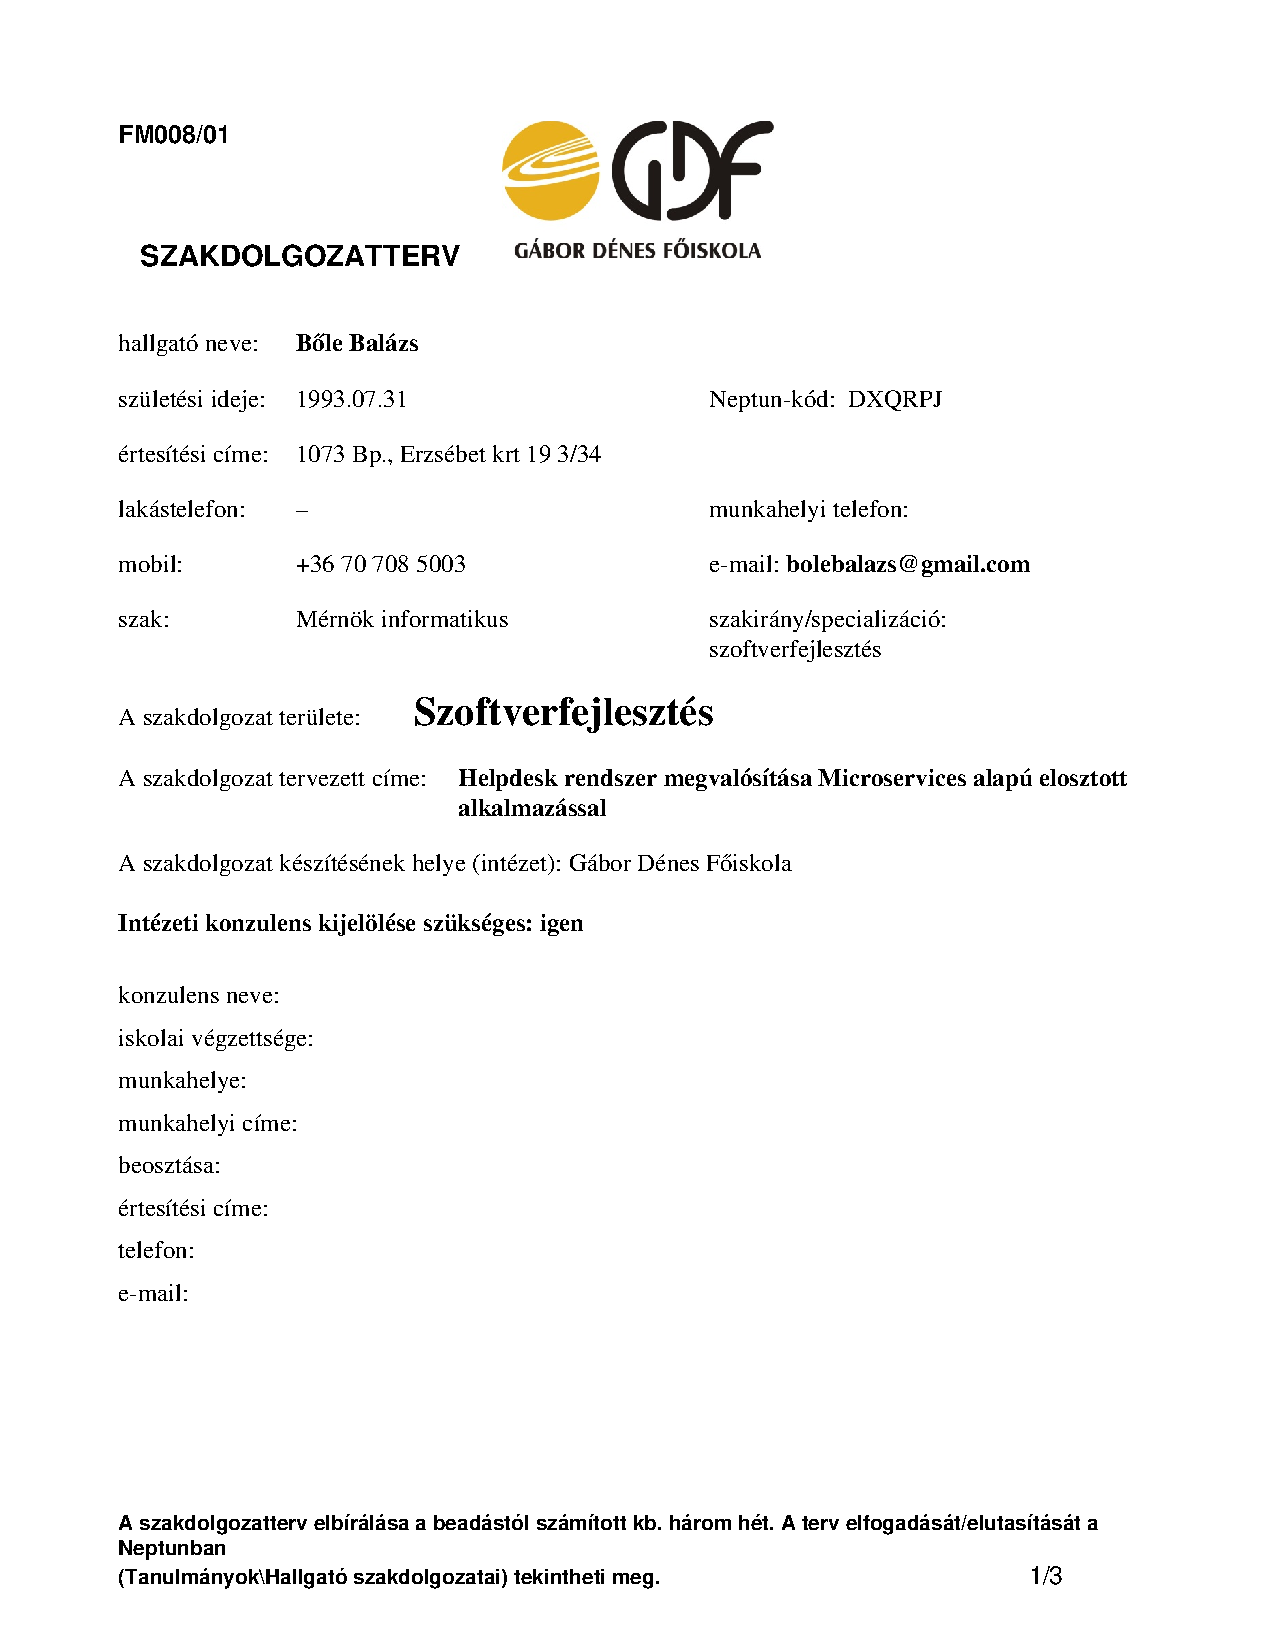
\includepdf[pages=-]{FM008_01_Szakdolgozatterv-DXQRPJ.pdf}
\cleardoublepage
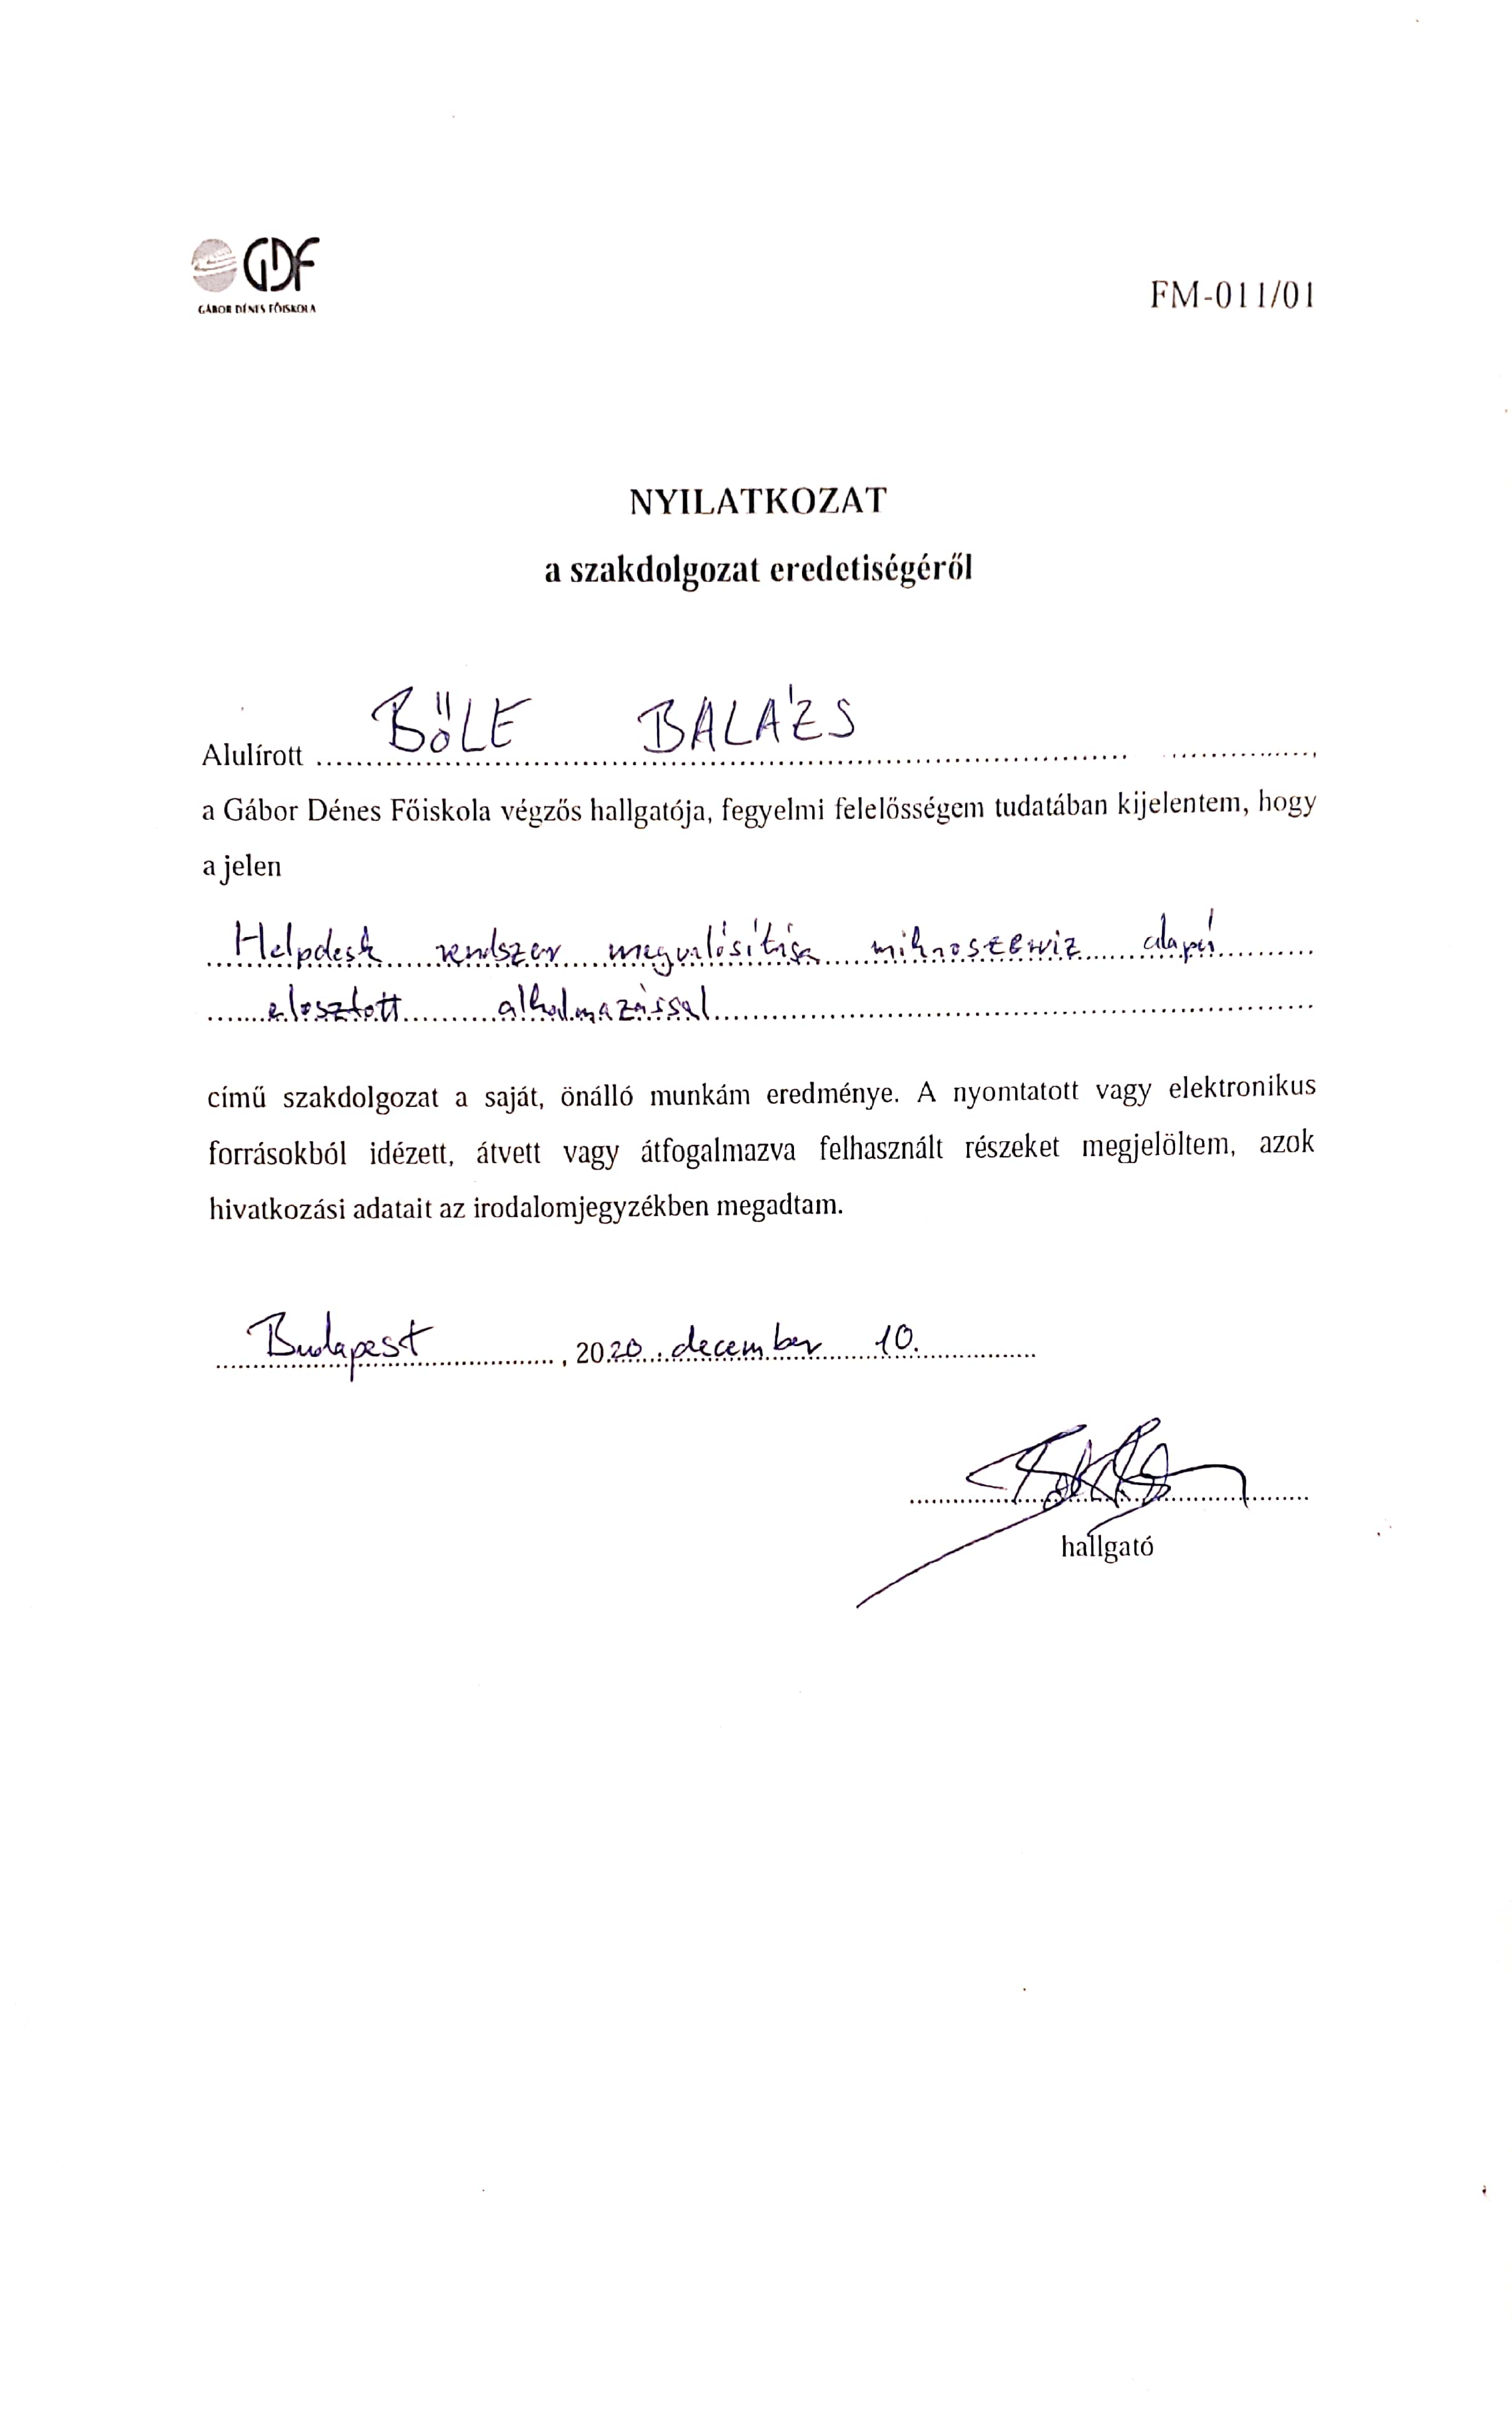
\includepdf[pages=-]{eredetiseg-nyilatkozat.pdf}

\thispagestyle{empty}
\cleardoublepage

\thispagestyle{empty}
\begin{center}
	{\Large \bfseries \@title}
	
	\bigskip
	\bigskip
	
	készítette
	
	\bigskip
	\bigskip
	
	{\large \bfseries \@author}
	
	\bigskip
	
	\vfill
	
	\begin{tabular}{ll}
		Neptun kód: & DXQRPJ \\
		Elérhetőség: & \href{mailto:bolebalazs@gmail.com}{bolebalazs@gmail.com}\\
		
		\bigskip\\
		
		Konzulens: & Dr.\ Nagy\ Elemér\ Károly
		

	\end{tabular}

	\bigskip
	\bigskip

\mbox{A dolgozat elektronikus változata elérhető a \url{https://github.com/balazsBole/} címen.}	
	

	
	\bigskip
	
	
\includegraphics[width=0.2\textwidth]{gdf_logo.png}

	
\end{center}
Budapest, \monthyeardate{\@date}.

\makeatother

\clearpage
\begin{abstract}
	Dolgozatomban ismertetem egy mikroszerviz alapú elosztott alkalmazás felépítését, a tervezés során fellépő általános problémákat, valamint ezekre a problémákra adható megoldásokat. 
	
	Nagy vonalakban és feladatspecifikusan áttekintem a felhasznált technológiákat és módszertanokat.
	
	Ezek tükrében bemutatom a létrehozott szoftvert,  infrastruktúrát és az üzemeltetéséhez szükséges eszközöket.
	
\end{abstract}

\pagestyle{front}
\tableofcontents

\begingroup
\let\clearpage\relax
\listoffigures
\endgroup


\clearpage
\pagenumbering{arabic}
\chapter*{Bevezetés}\label{ch:bevezetes}
	\addcontentsline{toc}{chapter}{\nameref{ch:bevezetes}}
Ahogy az \foreignlanguage{british}{O'Really} által az év elején készített felmérésből \cite{OReally} is látszik, a mikroszerviz alapú alkalmazások egyre nagyobb népszerűségnek örvendenek. Egyre több cég szeretné lecserélni meglévő monolit rendszerét, vagy a szükséges új funkciókat a régebbi rendszertől függetlenül, hibrid rendszerben valósítana meg.

Mint az a \foreignlanguage{british}{wiredelta} cikkéből \cite{wiredelta} is látszik, a mikroszerviz architektúrának számtalan előnye van. Míg a nagyvállalati környezetben sokszor a folyamatos szállítási igény, vagy az egymástól függetlenül fejleszthető alrendszerek miatt döntenek emellett a technológia mellett, az én esetemben a legfontosabb szerepet a skálázhatóság, az újrafelhasználhatóság, és  az alacsony fenntartási költség játszotta.

Úgy gondolom, hogy nincs olyan technológia, ami minden problémára megoldást nyújtana. De úgy érzem hogy az ilyen elvek mentén kialakított alkalmazások, természetükből adódóan időtállóbbak lesznek. Ha el tudjuk érni, hogy egy alkalmazás valóban csak egy funkcióért kell hogy felelős legyen, azzal a problémamegoldás analitikus oldalát  emeljük rendszerszintre. 

Éppen ezért, a mikroszerviz architektúra legnagyobb előnye szerintem a rendszerezésből következik.


\chapter{Üzleti igények}\label{ch:uzleti_igenyek}
\pagestyle{main}
\section{Funkcionális igények}



\section{Nem funkcionális igények}	


\chapter[Technológiai áttekintés]{Felhasznált technológiák}\label{ch:felhasznalt_technologiak}
\pagestyle{main}
Az alkalmazás rendszer szinten mikroszerviz (\ref{sec:mikroszerviz}), a modulok szintjén hexagonális architektúrába (\ref{sec:hexagonalis_architektura}) rendezve készült el. A frontend Angulart (\ref{sec:angular}), a backend és az e-mail kliens Spring Boot-ot (\ref{sec:spring_boot}) használ.


\section{Mikroszerviz architektúra}\label{sec:mikroszerviz}
Bár a kifejezés már régóta ismert, nincs egy központilag elfogadott, egységes definíció arra nézve, miket nevezünk mikroszervizeknek. A legtöbb szerző jobb híján a visszatérő karakterisztikus tulajdonságuk alapján sorolja be az alkalmazásokat ebbe a kategóriába~\cite{OReally_Microservice_Architecture}. Egy tipikus mikroszerviz a következő tulajdonságoknak felel meg:

\begin{itemize}
	\item	pontosan egy üzleti funkció köré szerveződik 
	\item   más	szervizekkel laza, általában hálózaton keresztül megvalósuló kapcsolatban áll
	\item   ha szüksége van adatbázisra, akkor sajáttal rendelkezik
	\item	önmagában is működőképes	
	\item	decentralizált, tehát nincs egy a munkáját befolyásoló központi irányítórendszer
\end{itemize}

A hasonló felépítésükből adódóan, számos olyan eszköz van, ami --nem kötelezően, de legtöbbször-- együtt fordul elő a mikroszerviz architektúrával. A legfontosabb ilyen fogalmak a:
\begin{description}
	\item[skálázhatóság] a rendszer képessége az áteresztőképességének növelésére.
	Létezik vertikális\footnote{több processzor vagy memória bevonása} és horizontális skálázhatóság\footnote{újabb példányok futtatása}.
	
	\item[konténerizálás] a szerviz futtatása saját elszeparált környezetében hardveres virtualizáció segítsége nélkül.	

	\item[erőforrás felderítés] a rendszer által nyújtott erőforrások automatikus
	felfedezhetősége\footnote{angolul \textit{service discovery}-nek hívják}.
	
	\item[loadbalancer] az a folyamat, ami a bejövő feladatokat erőforrásokhoz rendeli. Legegyszerűbb megvalósítása a \foreignlanguage{british}{\textit{round robin}} algoritmus, célja a terhelés egyforma elosztása.
	
	\item[monitorozás] az önálló szervizek állapotának felügyelése. A monitorozás során nyújtott metrikák kiterjedhetnek a felhasznált memória mennyiségére, processzorigényére, vagy processzeire is.
\end{description}


\section{Hexagonális architektúra}\label{sec:hexagonalis_architektura}
A hexagonális architektúra --vagy más néven portok és adapterek architektúrája-- egy \foreignlanguage{british}{Alistair Cockburn} által létrehozott \cite{Alistair_Cockburn} szoftverterezési minta. Nevét a cikkben felrajzolt hatszögletű rendszerábrázolásról kapta (\ref{fig:Alistair_Cockburn_hexagonal_architecture} ábra), ami szembemegy a korábban elterjedt réteges elrendezéssel.

Az eredeti szándék mögötte az alkalmazás függetlenítése mindennemű külső függőségtől\footnote{például adatbázis, felhasználók, automatizált tesztek}, így lehetővé téve az üzleti és a technikai igények nagy mértékű szeparálását.
Egy absztrakt port feladata kell legyen a külvilággal való kapcsolat, így az üzleti logika csak az üzenet tartalmáért felelős, az üzenetküldés módjáért már nem.

\begin{figure}[hbt] 
	\centering
		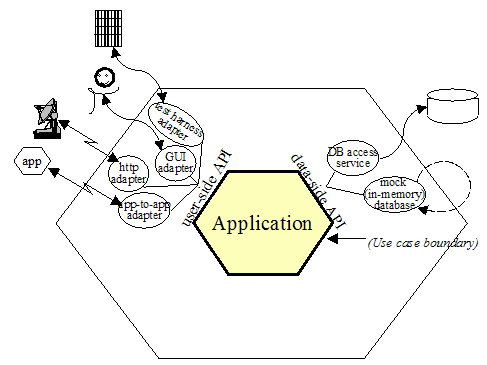
\includegraphics[width=0.85\textwidth]{Alistair_Cockburn_hexagonal_architecture.png}
	\caption[Hexagonális alkalmazások felépítése]{\foreignlanguage{british}{Alistair Cockburn} által \cite{Alistair_Cockburn} felrajzolt ábra a hexagonális alkalmazásról. Cockburn célja a külső függőségek elszeparálásának bemutatása.
}\label{fig:Alistair_Cockburn_hexagonal_architecture}
\end{figure}

Ahogy \foreignlanguage{british}{Robert C. Martin} a \foreignlanguage{british}{\textit{The Clean Architecture}} cikkében \cite{The_Clean_Architecture} összeszedte, a port-adapter és a hasonló architektúrával készülő alkalmazások mind:	
\begin{itemize}
	\item Könnyen, és önmagukban is tesztelhetőek. Mivel az üzleti szabályoknak, nincs külső függőségük.
	
	\item Függetlenek a külső tényezőktől. Így az alkalmazás által használt felület vagy adatbázis könnyen cserélhető.
	
	\item Keretrendszertől függetlenül is megvalósíthatóak. A megvalósítás nem függ semmilyen könyvtártól vagy egyéb tulajdonságtól.
\end{itemize}
	
	

\section{Event stream processing}
adatvezérelt, event based, szeparálás miatt 
publish subscribe
 schema
 kafka\\
event processiing általánosan?


\section{Rétegek szeparálása}\label{sec:retegek_szeparalasa}
A hexagonális architektúra (\ref{sec:hexagonalis_architektura} pont) és a hasonló \textit{clean code} \cite{clean_code_chapter_systems} elvek sokszor a különböző szoftver rétegek elkülönítésén alapszanak.


Hogy a feladatok elkülönítése ne vonzza magával az ismétlődő program részletek megnövekedését, célszerű a visszatérő, üzleti funkciót nem hordozó sorokat generálni. Ilyen --a fordítási időben-- kódot generáló eszközök a Mapstruct és a Lombok.


\section{Angular}\label{sec:angular}
Az \foreignlanguage{british}{Angular} egy a \foreignlanguage{british}{Google} által fejlesztett \foreignlanguage{british}{TypeScript} alapú platform és		 keretrendszer~\cite{angular_docs}. A segítségével létrehozott kód erősen modularizált, így könnyű vele újra felhasználható és az MVC-elveit követő alkalmazást létrehozni.

A segítségével készített honlap teljes mértében a kliens oldalon fut, így a szerver oldalon elegendő egy egyszerű, statikus HTML-oldalt visszaadó alkalmazásszerver használata.


\section{Spring Boot}\label{sec:spring_boot}
A \foreignlanguage{british}{Spring Boot} egy a Springre épülő keretrendszer. Mindkét rendszer alapja a függőség befecskendezése\footnote{Angolul \foreignlanguage{british}{\textit{Dependency Injection}}}, ami egy \aref{sec:retegek_szeparalasa} pontban említett tiszta kód \cite{clean_code_chapter_systems} eszköze.

A Spring Boot \cite{introducing_spring_boot} célja hogy gyorsan és egyszerűen lehessen önálló, magas minőségű alkalmazásokat fejleszteni:
\begin{itemize}
	\item az alapbeállítástól való eltérést kell meghatározni\footnote{A Spring Boot dokumentációban ezt röviden \textit{convention over configuration}-nek hívják} ezzel lecsökkentve a konfigurációval töltött időt,
	\item valamint sok gyakran visszatérő problémára\footnote{Például: metrikák, biztonság, adattárolás} nyújt könnyen elérhető megoldást.
\end{itemize}






\chapter{Az alkalmazás felépítése}\label{ch:felepites}
\pagestyle{main}
Ebben a fejezetben átfogó képet adok az általam létrehozott helpdesk alkalmazásról. Az egyes komponensek részletes leírása \aref{ch:implementacio}. fejezetben található.

\section{Legfontosabb komponensek}

\begin{figure}[hbt] 
	\centering
	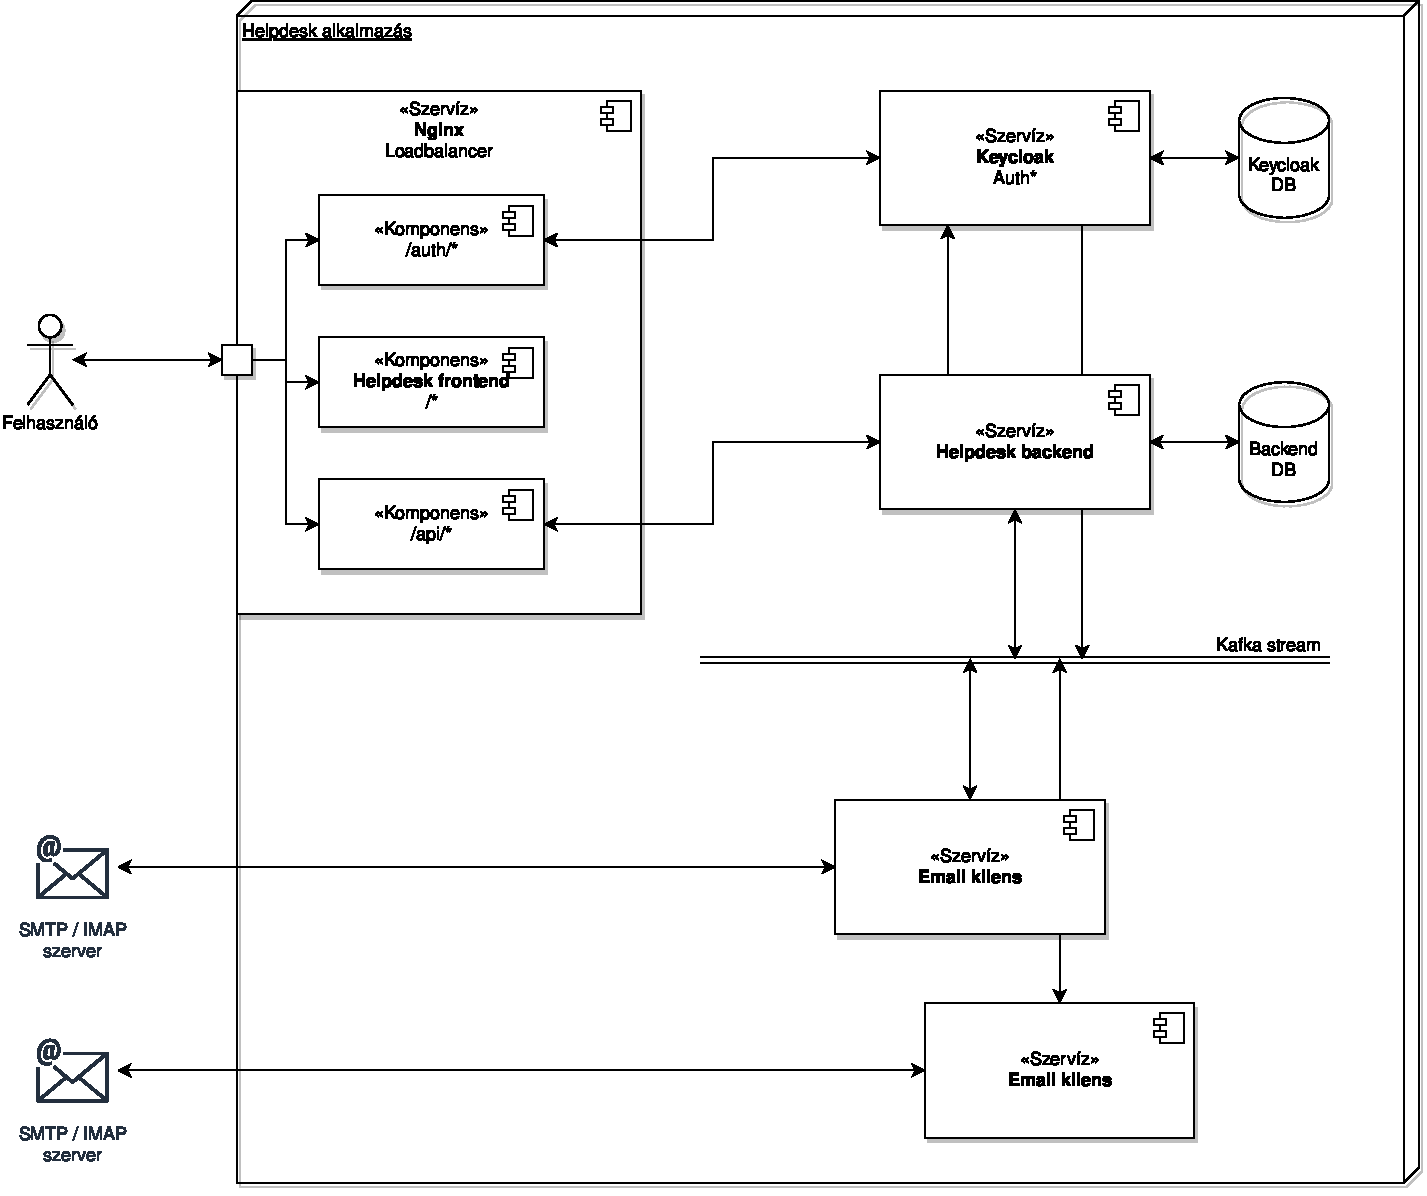
\includegraphics[width=0.87\textwidth]{komponens_diagram_drawio.pdf}
	\caption{A legfontosabb komponensek}
	\label{fig:komponens_diagram}
	\floatfoot{Forrás: saját ábra}
\end{figure}

\Aref{fig:komponens_diagram}. ábrán a legfontosabb szolgáltatásokat gyűjtöttem össze. Az üzleti funkcionalitás megvalósulása az itt bemutatott komponensek összehangolt munkáján keresztül valósul meg.



\begin{itemize}
	\item A felhasználó az nginx-en (\ref{sec:nginx} pont) keresztül éri el a heldesk alkalmazást.
	\item Az nginx dönti el, hogy melyik URL-t melyik szolgáltatás szolgálja ki.
	\item Az email kliens és a heldpesk backend kafka streamen keresztül éri el egymást.
	\item Az email kliensek kezelik az e-mail szerverekkel való adatcserét.
\end{itemize}


\section{Adatbázis UML diagram}\label{sec:felepites_adatbazis}
A helpdesk backend adatbázis legfontosabb tábláit \aref{fig:basic_database_uml}. ábra tartalmazza. Az ábrán nem szerepelnek az audit és a Liquibase által használt táblák~(\ref{sec:adatbazis} pont). \Aref{ch:bemutatas}. fejezetben található \ref{fig:extended_database_uml}. ábra tartalmazza az adatbázis összes tábláját.
 


\begin{figure}[hbt] 
	\centering
	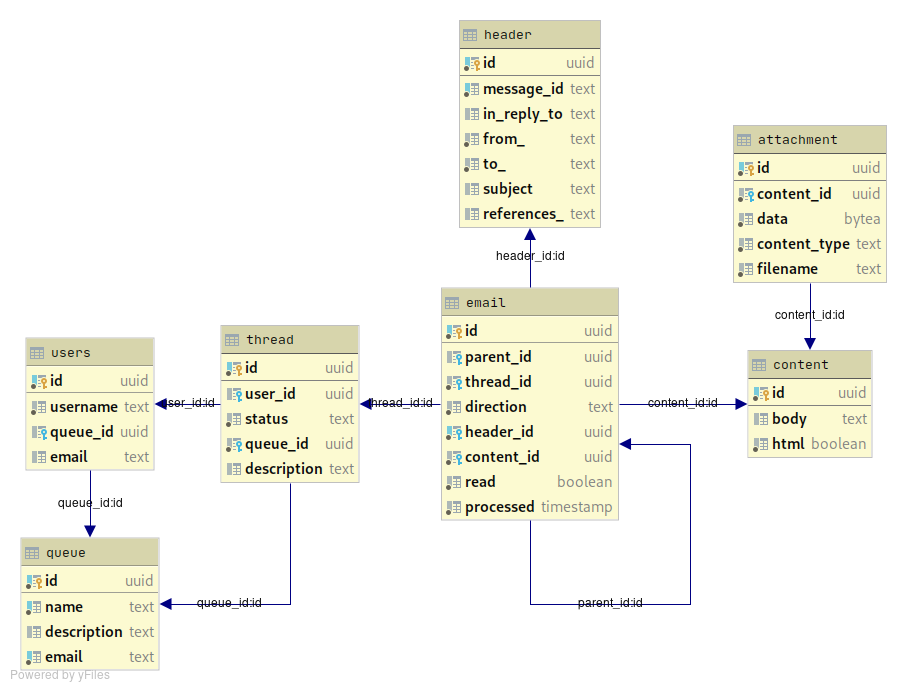
\includegraphics[width=0.85\textwidth]{basic_database_uml.png}
	\caption{A backend legfontosabb adatbázistáblái}
	\label{fig:basic_database_uml}
	\floatfoot{Forrás: saját ábra}
\end{figure}

\section{E-mail fogadásának és küldésének folyamata}
A könnyebb átláthatóság érdekében, a folyamatokat egy e-mail szemszögéből mutatom be \aref{fig:path_of_an_email}. ábrán. Az e-mail fogadása az alábbi felsorolás által leírt folyamat szerint történik.
\begin{enumerate}
	\item Az e-mail kliens IMAP protokollon keresztül megkapja az új e-mailt.
	\item Az e-mail kliens a bejövő e-mailt egy kafka üzenetként teszi közzé a bejövő e-mailek kafka \emph{topicban}.
	\item A bejövő e-mailek \emph{topic}ra feliratkozott helpdesk backend megkapja a kafka üzenetet.
	\item A helpdesk backend eltárolja az új üzenetet az adatbázisban
	\item A felhasználó a frontend segítségével lekérdezi az újonnan beérkezett e-maileket.
	\item A helpdesk backend a kérésre elküldi az újonnan fogadott e-mailt.
\end{enumerate}

\bigskip
Az email küldése pedig az alábbi felsorolás szerint hajtódik végre.
\begin{enumerate}
	\item A felhasználó az új e-mail elolvasása után a frontend segítségével megírja a választ.
	\item A felhasználó elküldi a választ a helpdesk backendnek.
	\item A helpdesk backend eltárolja az adatbázisba az új e-mailt, majd az e-mail szálnak megfelelő kimenő e-mail \emph{topic}ba közzéteszi az új üzenetet.
	\item Az e-mail cím specifikus kimenő e-mailek \emph{topic}ra feliratkozott e-mail kliens megkapja a kafka üzenetet.
	\item Az e-mail kliens SMTP protokollon keresztül elküldi az új e-mailt.
\end{enumerate}


\begin{figure}[hbt] 
	\centering
	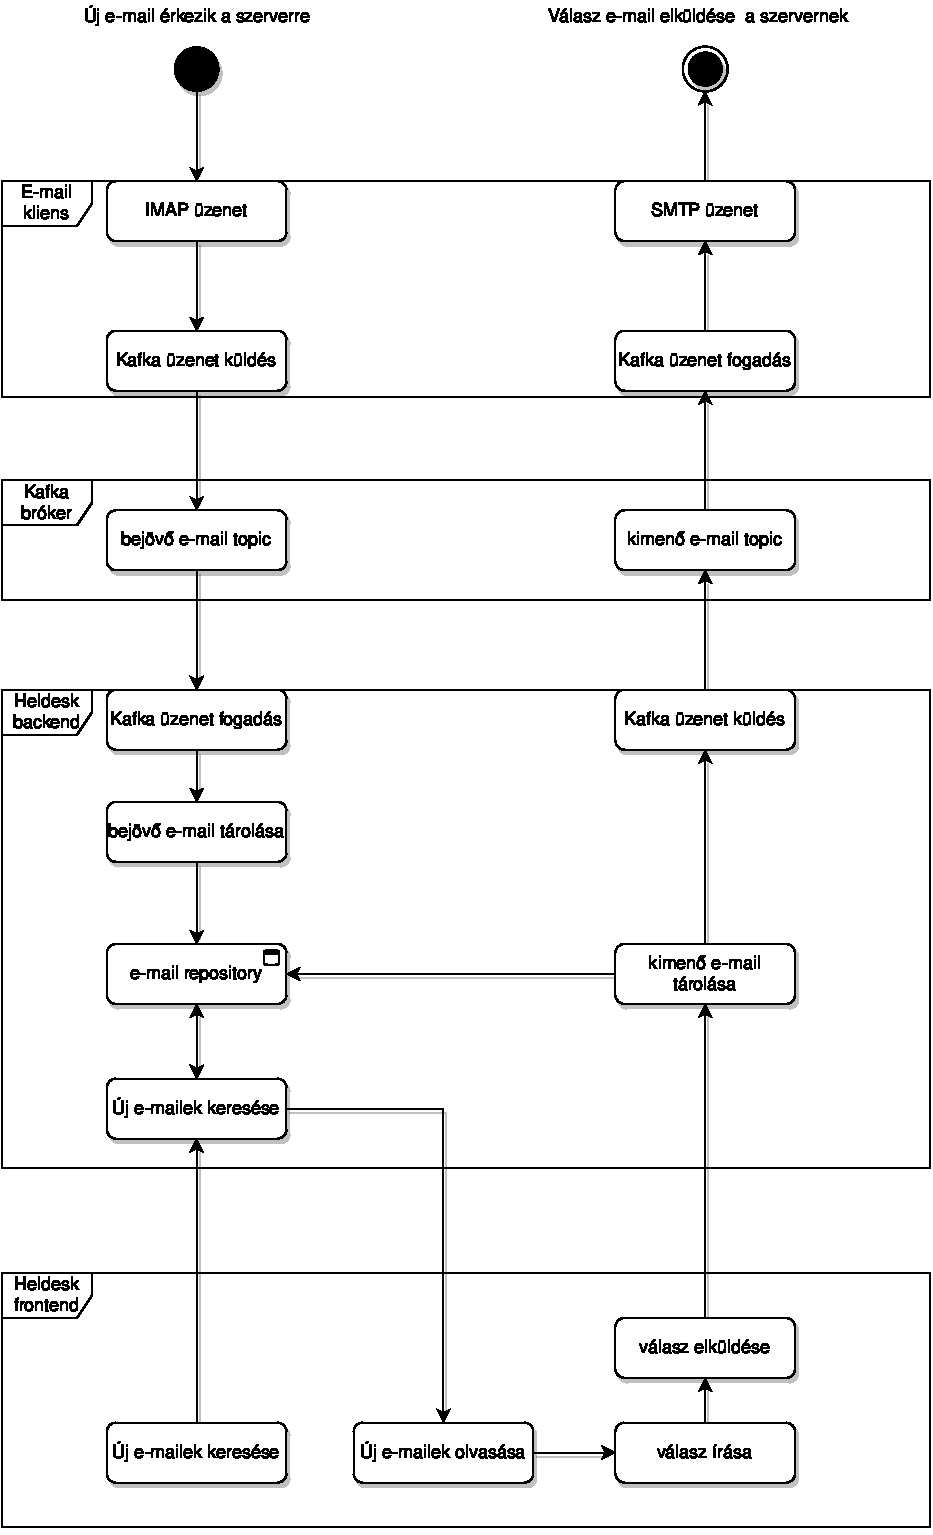
\includegraphics[width=0.7\textwidth]{path_of_an_email_drawio.pdf}
	\caption{A bejövő és kimenő e-mail útja}
	\label{fig:path_of_an_email}
	\floatfoot{Forrás: saját ábra}
\end{figure}



\chapter{Implementáció}\label{ch:implementacio}
\pagestyle{main}
\section{Mikroszerviz infrastruktúra}

\subsection{Nginx}
Az nginxnek három elkülönülő szerepe van:

\begin{itemize}
	\item{A \foreignlanguage{british}{helpdesk frontend} alkalmazásszervereként működik (lásd \ref{sec:angular} pont)}
	
	\item{\foreignlanguage{british}{Routing}ot valósít meg, rajta kerestül érhető el a \foreignlanguage{british}{helpdesk backend} és a \foreignlanguage{british}{keycloak} szerviz}
	
	\item{\foreignlanguage{british}{HTTP cahce}-ként működik a frontend és a backend között, illetve a frontend és a keycloak között}
\end{itemize}

A loadbalancer funkcionalitás a \foreignlanguage{british}{docker round-robin DNS}-én (\ref{sec:docker}) keresztül valósul meg.


\subsection{Docker konténerizáció}\label{sec:docker}
Az alakalmazás összes szervize saját docker konténerben fut. A docker konfigurációs leírása a \textit{docker-compose.yml} állományban van. A \textit{docker-compose} parancs ez alapján indítja el az alkalmazást, hozza létre a saját alhálózatát, valósítja meg a hálózaton belüli DNS-funkciót.

A konténerek skálázása  is a dockeren keresztül (\textit{docker-compose --scale}) valósul meg.



\subsection{metrikák}
A springes alkamazásaim egy-egy HTTP endpointon keresztül érhetőek el a prometheus számára (\textit{\mbox{/actuator/proemtheus}}) és induláskor beregisztrálják magukat az eureka szerverbe\footnote{Az Eureka a Netflix által fejlesztett \textit{discovery server}. Feladata az összes kliens port és ip adatának nyilkvántartása.}.

A prometheus\footnote{A Prometheus egy open source monitorozó eszköz. 15 másodpercenként lekérdezi a szervizek állapotát.} az eurekán keresztül találja meg az instanceokat, és gyűjti össze a metrikákat. Az alkalmazások információt küldenek a Kafka konnektorukról, REST interfészükről és az adatbázis kapcsolatukról\footnote{HikariCP-t használok JDBC kapcsolathoz}.

A Prometheus által összegyűjtött adatokat grafanában\footnote{A Grafana egy open source elemző és megjelenítő web alkalmazés} ábrázolom.






\section{E-mail kliens}
Az e-mail kliens szerepe az üzenetek küldése és fogadása egy meghatározott e-mail címről. Feladata a külső protokollok leválasztása az alkalmazástól. Irányítja és karbantartja az IMAP és SMTP szerverrel való kapcsolatot.

A két irányú kömmunikáció megvalósulása:
\begin{enumerate}
	\item az IMAP-on keresztül fogadott e-mailt az \textit{email.in.v1.pub} kafka topicba írja
	\item a saját --e-mail cím specifikus-- topic-jából kiolvassa az üzenetet és továbbítja  az SMTP szerver felé
\end{enumerate}

\subsection{E-mail szabvány}

	rfc5322: 
	messageId
	replyTo
	refereneces







\section{helpdesk backend}
Class Diagram

\subsection{springBoot}
default behavior, DI
security, 	

\subsection{data persistance layer}
hibernate, liquibase, Hibernate envers (Auditlog)

\subsection{egyéb eszközök}
openApi dokumnetáció, mapstruct, hibernate, lombok






\section{helpdesk frontend}
MVC szerint van szeparálva a kód 	

\subsection{RxJs store}

\subsection{Komponensek}
material, quill

\subsection{deploymnet}
static html-lé fordul a kliens oldalán fut a frontend






\section{keycloak}	
\subsection{JWT-token}
\subsection{role-ok}
\subsection{admin felületről valami?}


\chapter{Alkalmazás bemutatása}\label{ch:bemutatas}
\pagestyle{main}
A helpdesk alkalmazás \aref{ch:uzleti_igenyek}. fejezetben leírtaknak megfelelően szolgál ki három különböző e-mail címet:

\begin{itemize}
	\item a \textit{generic} sorhoz tarozó  \href{mailto:helpdesk.gdf@yandex.com}{\nolinkurl{helpdesk.gdf@yandex.com}}-ot, 
	\item a \textit{travel} sorhoz tarozó  \href{mailto:helpdesk.gdf.travel@yandex.com}{\nolinkurl{helpdesk.gdf.travel@yandex.com}}-ot,
	\item és a \textit{theater} sorhoz tarozó  \href{mailto:h.gdf.theater@gmx.com}{\nolinkurl{h.gdf.theater@gmx.com}}-ot.
\end{itemize}



\section{Alkalmazás elindítása}\label{sec:elinditas}
Az alkalmazás a \textit{start.sh} bash \textit{script}tel indítható el. A \textit{script} két dolgot csinál:
\begin{enumerate}
	\item a \textit{docker-compose} parancssal elindítja a docker \textit{container}eket~(\ref{sec:docker} pont),
	\item  ``helpdesk'' domain névvel hozzáadja az Nginx (\ref{sec:nginx} pont) IP címét a \mbox{\textit{/etc/hosts}} állományhoz.
\end{enumerate}

A \textit{script} indítása után a helpdesk alkalmazás elérhető a  \href{http://helpdesk}{http://helpdesk} domain alatt.


\section{Deployment}
A könyebb bemutathatóság érdekében a szemléletesebb szervizeket --  hogy ne a docker daemon által kiosztott IP címen keresztül kelljen elérni --   a docker hálózaton kívül is elérhetővé tettem. 

A \textit{docker-compose} (\ref{sec:elinditas}) által elindított \textit{container}eket \aref{fig:deployment_diagram}. ábrán foglaltam össze. Az ábrán feltüntettem, hogy az adott \textit{container}t a \textit{localhost} melyik portján lehet elérni.


\begin{figure}[hbt] 
	\centering
	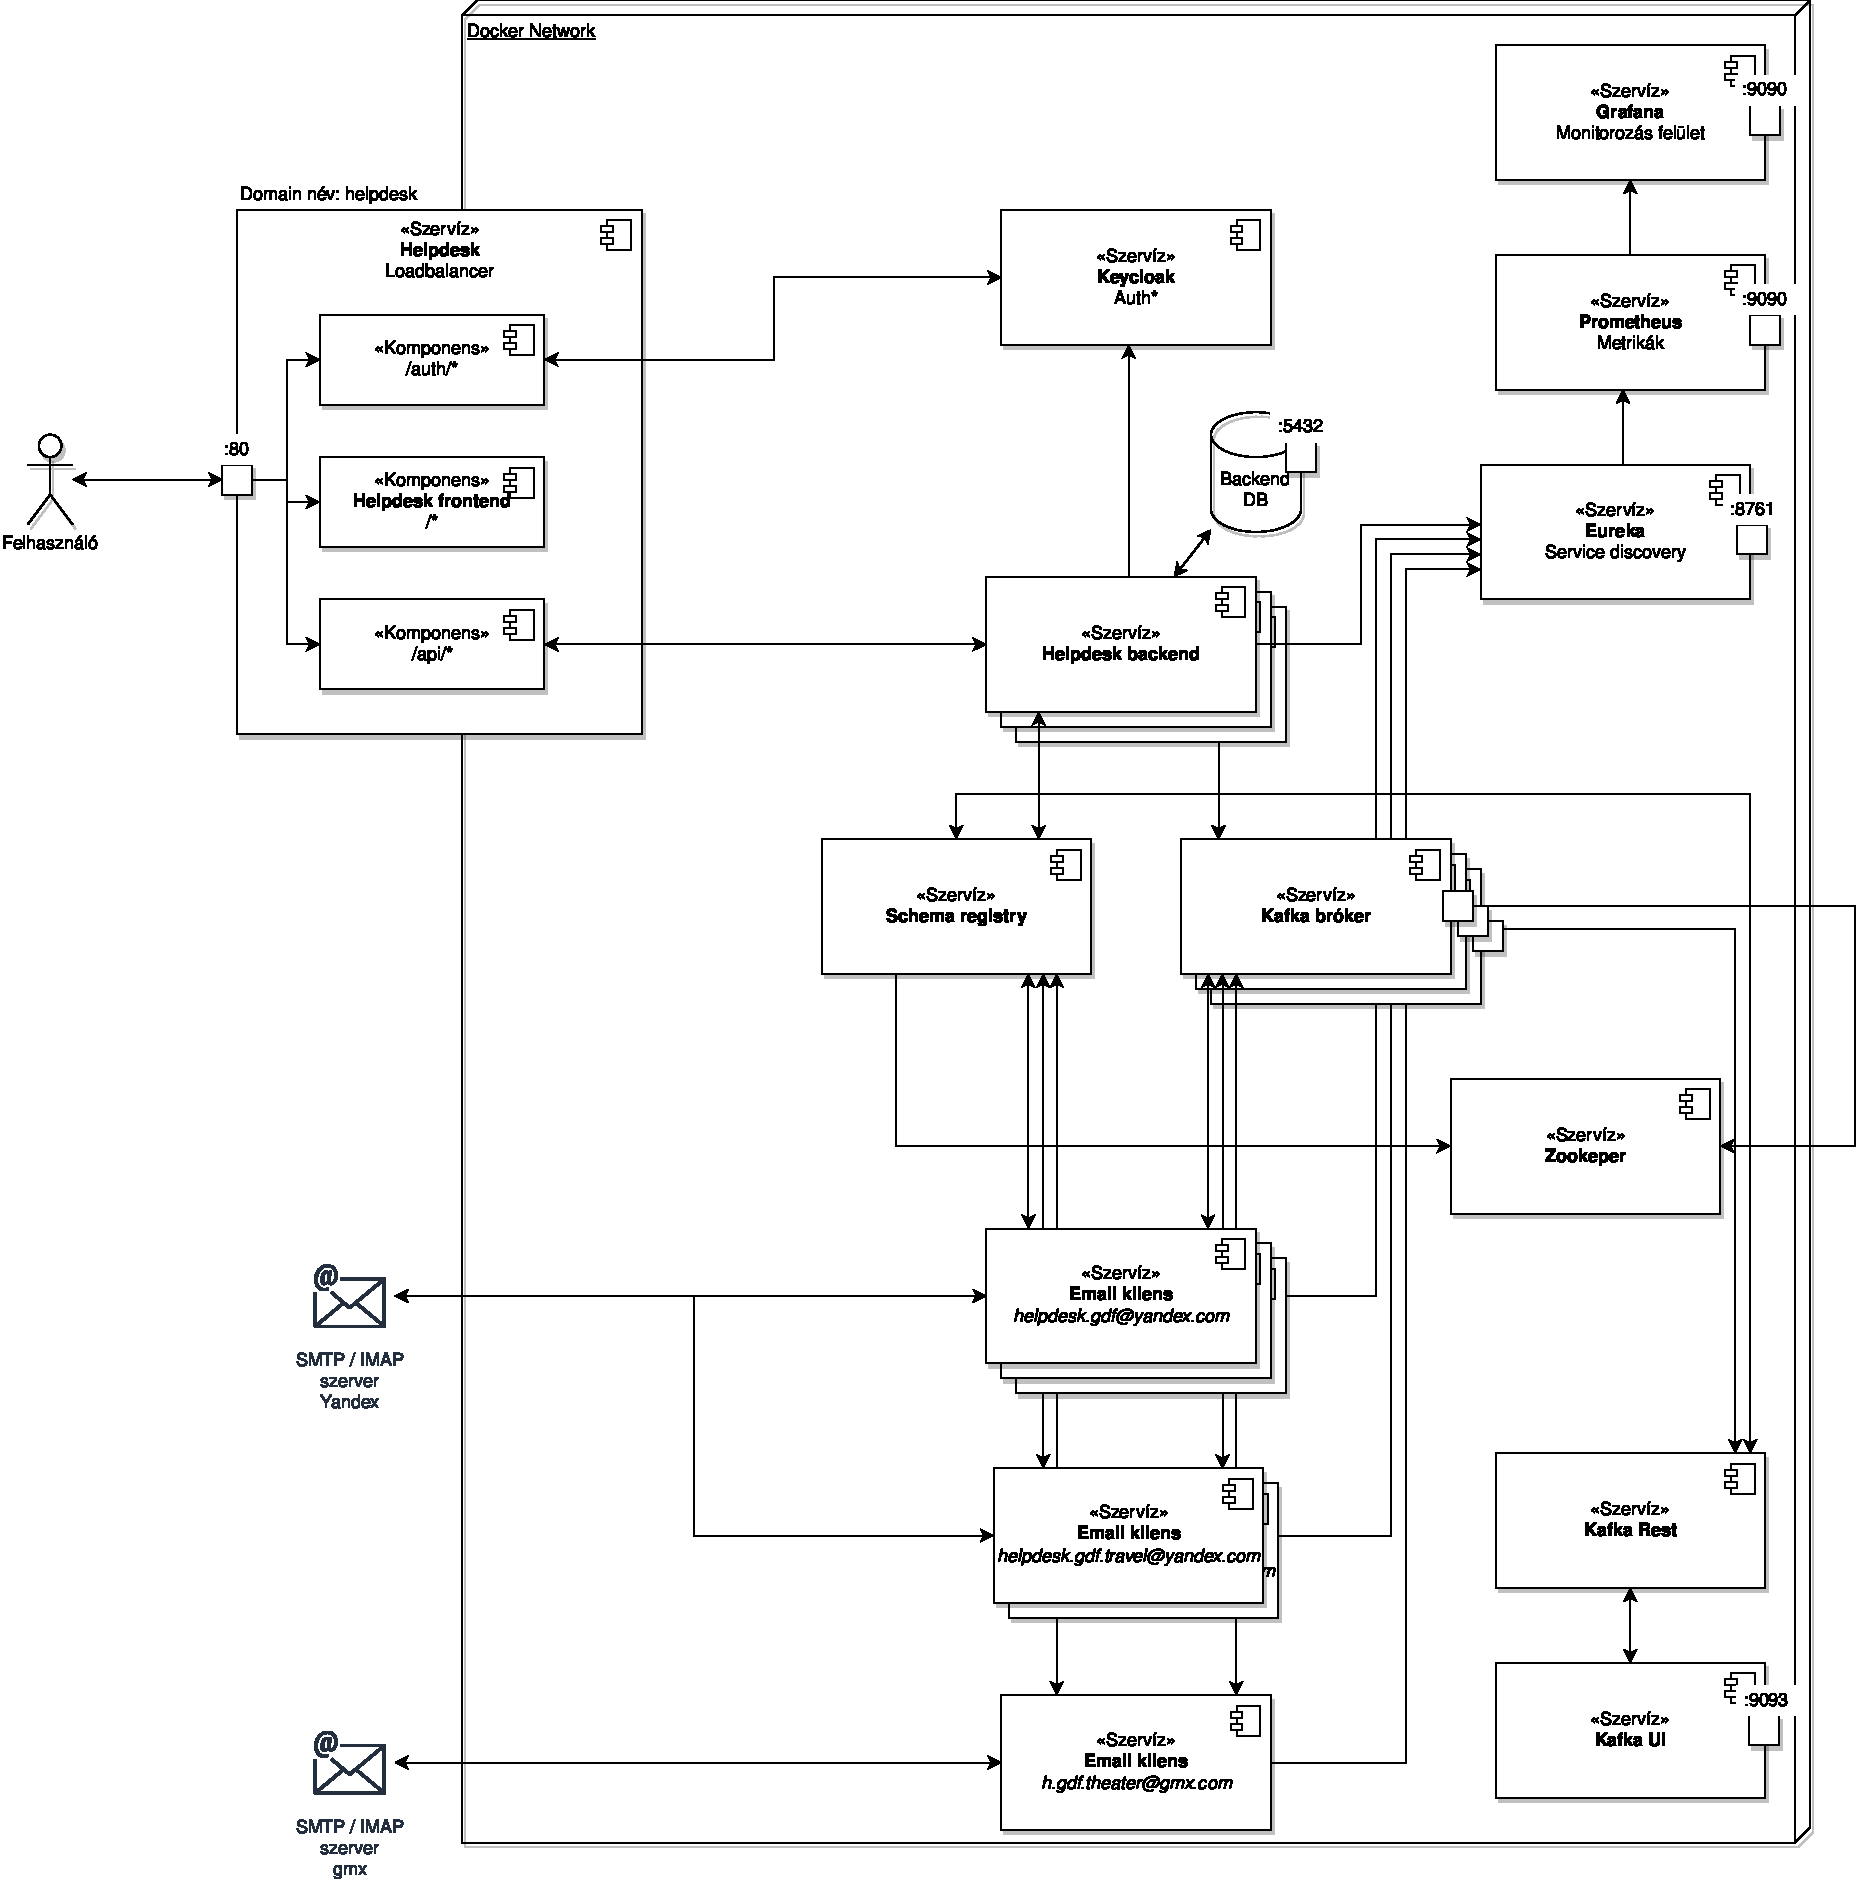
\includegraphics[width=0.95\textwidth]{deployment_diagram_drawio.pdf}
	\caption[Deployment diagram]{Deployment diagram}
	\label{fig:deployment_diagram}
	\floatfoot{Forrás: saját ábra}
\end{figure}



\section{Több példány}
A különböző szervizekből a terhelésnek megfelelően eltérő számú példány indul el:

\begin{itemize}
	\item a helpdesk-backendből három,
	\item a \textit{theater} sort kezelő email-kliensből egy,
	\item a \textit{travel} sort kezelő email-kliensből kettő,
	\item a \textit{generic} sort kezelő email-kliensből három,
	\item és a Kafka brókerből (\ref{sec:kafka_topics}) szintén három darab.
\end{itemize}

A példányok metrikáit (\ref{sec:metrikak} pont) nyomon lehet követni az erre a célra létrehozott Grafana oldalon (\ref{fig:backend_receive_kafka} ábra). Az oldal elérhető a  \textit{Spring metrics} menüpont alatt.

\Aref{fig:backend_receive_kafka} ábrán csak a Grafana oldal legfelső néhány panele látható, az instance-okra lebontott legfontosabb mérőszámokkal:

\begin{itemize}
	\item a legfelső sorban a Java Virtual Machine, által aktuálisan felhasznált Heap space,	
	\item alatta a feldolgozott Kafka üzenetek száma,
	\item a harmadik sorban a Trace log bejegyzések száma,
	\item míg az utolsó sorban az aktuális REST lekérések száma látható.
\end{itemize}



\section{E-mail fogadásának és küldésének folyamata}
\Aref{ch:felepites}. fejezetben \aref{fig:path_of_an_email}. ábrán bemutattam egy e-mail fogadásának elméleti útját. Most \aref{fig:email_send_receive_visible}. ábrán bemutatom hogyan követhető végig a rendszerben egy e-mail valódi útja.

E-mail fogadása:
\begin{enumerate}
	\item Egy teszt üzenet érkezik a \href{mailto:helpdesk.gdf.travel@yandex.com}{\nolinkurl{helpdesk.gdf.travel@yandex.com}} címre
	\textit{E-mail fogadásának és küldésének folyamata} tárggyal.
	\item Az e-mail kliens kafka üzenetként publikálja az üzenetet az \textit{email.in.v1.pub} topicba (\ref{fig:email_client_send_kafka}. ábra).
	\item A backend megkapja a kafka üzenetet (\ref{fig:backend_receive_kafka}. ábra).
	\item A backend elmenti az új üzenet az adatbázisba (\ref{fig:datbase_received_email}. ábra).
	\item A felhasználói felületen (\ref{fig:frontend_read_email}. ábra) elérhető az új üzenet.
\end{enumerate}

\bigskip

E-mail küldése:
\begin{enumerate}
	\item A felhasználó elküldi a válaszát a felhasználói felületen (\ref{fig:frontend_send_answer}. ábra).
	\item A backend megkapja az üzenetet és eltárolja az adatbázisba (\ref{fig:database_answer}. ábra).
	\item A \textit{h.gdf.theater\textunderscore gmx.com.v1.pub} topicban megjelenik. (\ref{fig:kafka_topic_send_email}. ábra) a backend által publikált kafka üzenet.
	\item A topicra feliratkozott e-mail kliens fogadja és továbbítja az üzenetet. (\ref{fig:email_client_receives_kafka}. ábra).
\end{enumerate}
 

\begin{figure}
	\begin{subfigure}{.49\textwidth}
		\centering
		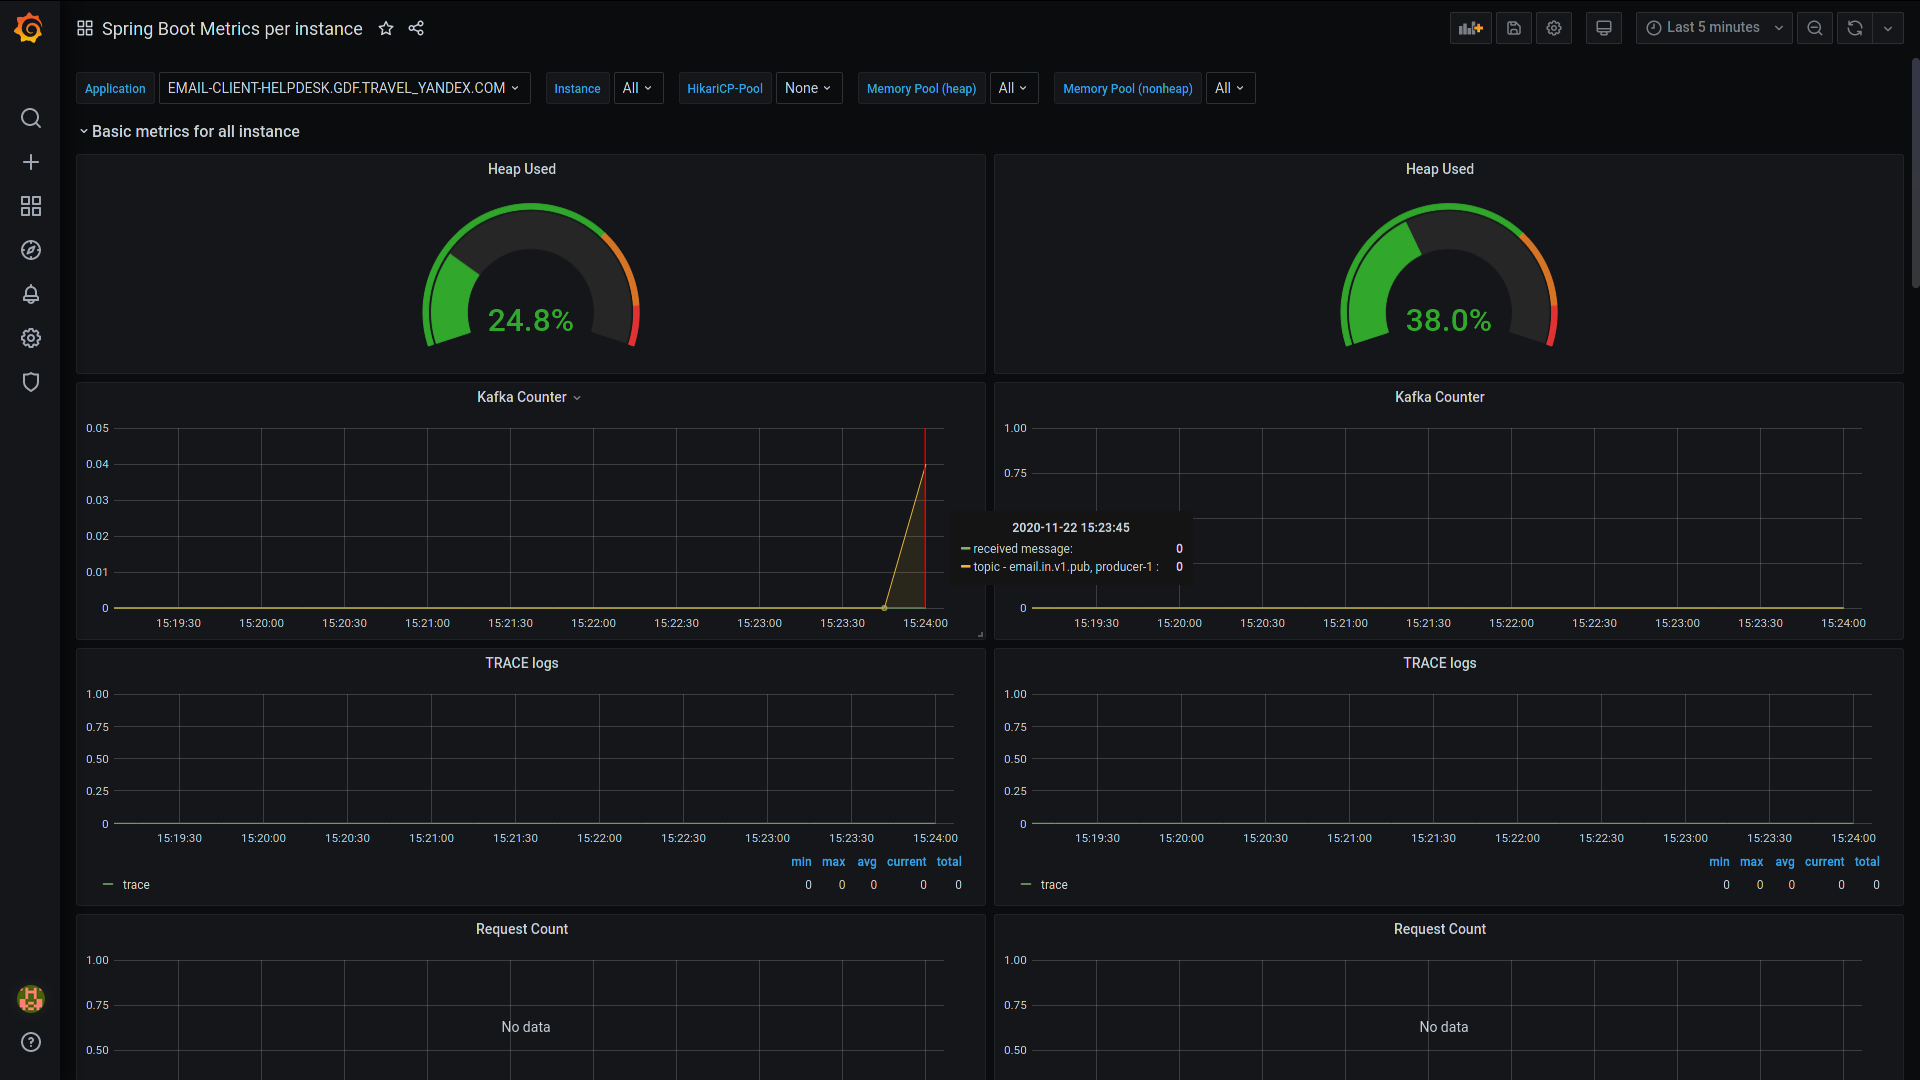
\includegraphics[width=.9\linewidth]{email_client_sending_kafka_message.png}  
		\caption{Az egyes instance kafka üzenet küld}
		\label{fig:email_client_send_kafka}
	\end{subfigure}
	\begin{subfigure}{.49\textwidth}
		\centering
		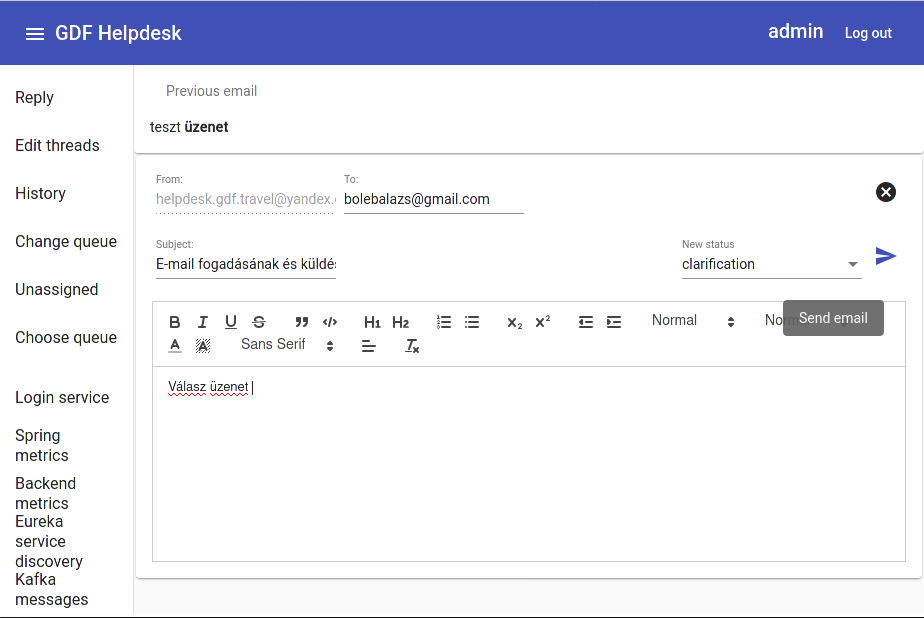
\includegraphics[width=.9\linewidth]{helpdesk_frontend_send_email.png}  
		\caption{A felületen válasz e-mailt küld a felhasználó}
		\label{fig:frontend_send_answer}
	\end{subfigure}
	
	\quad
	
	\begin{subfigure}{.49\textwidth}
		\centering
		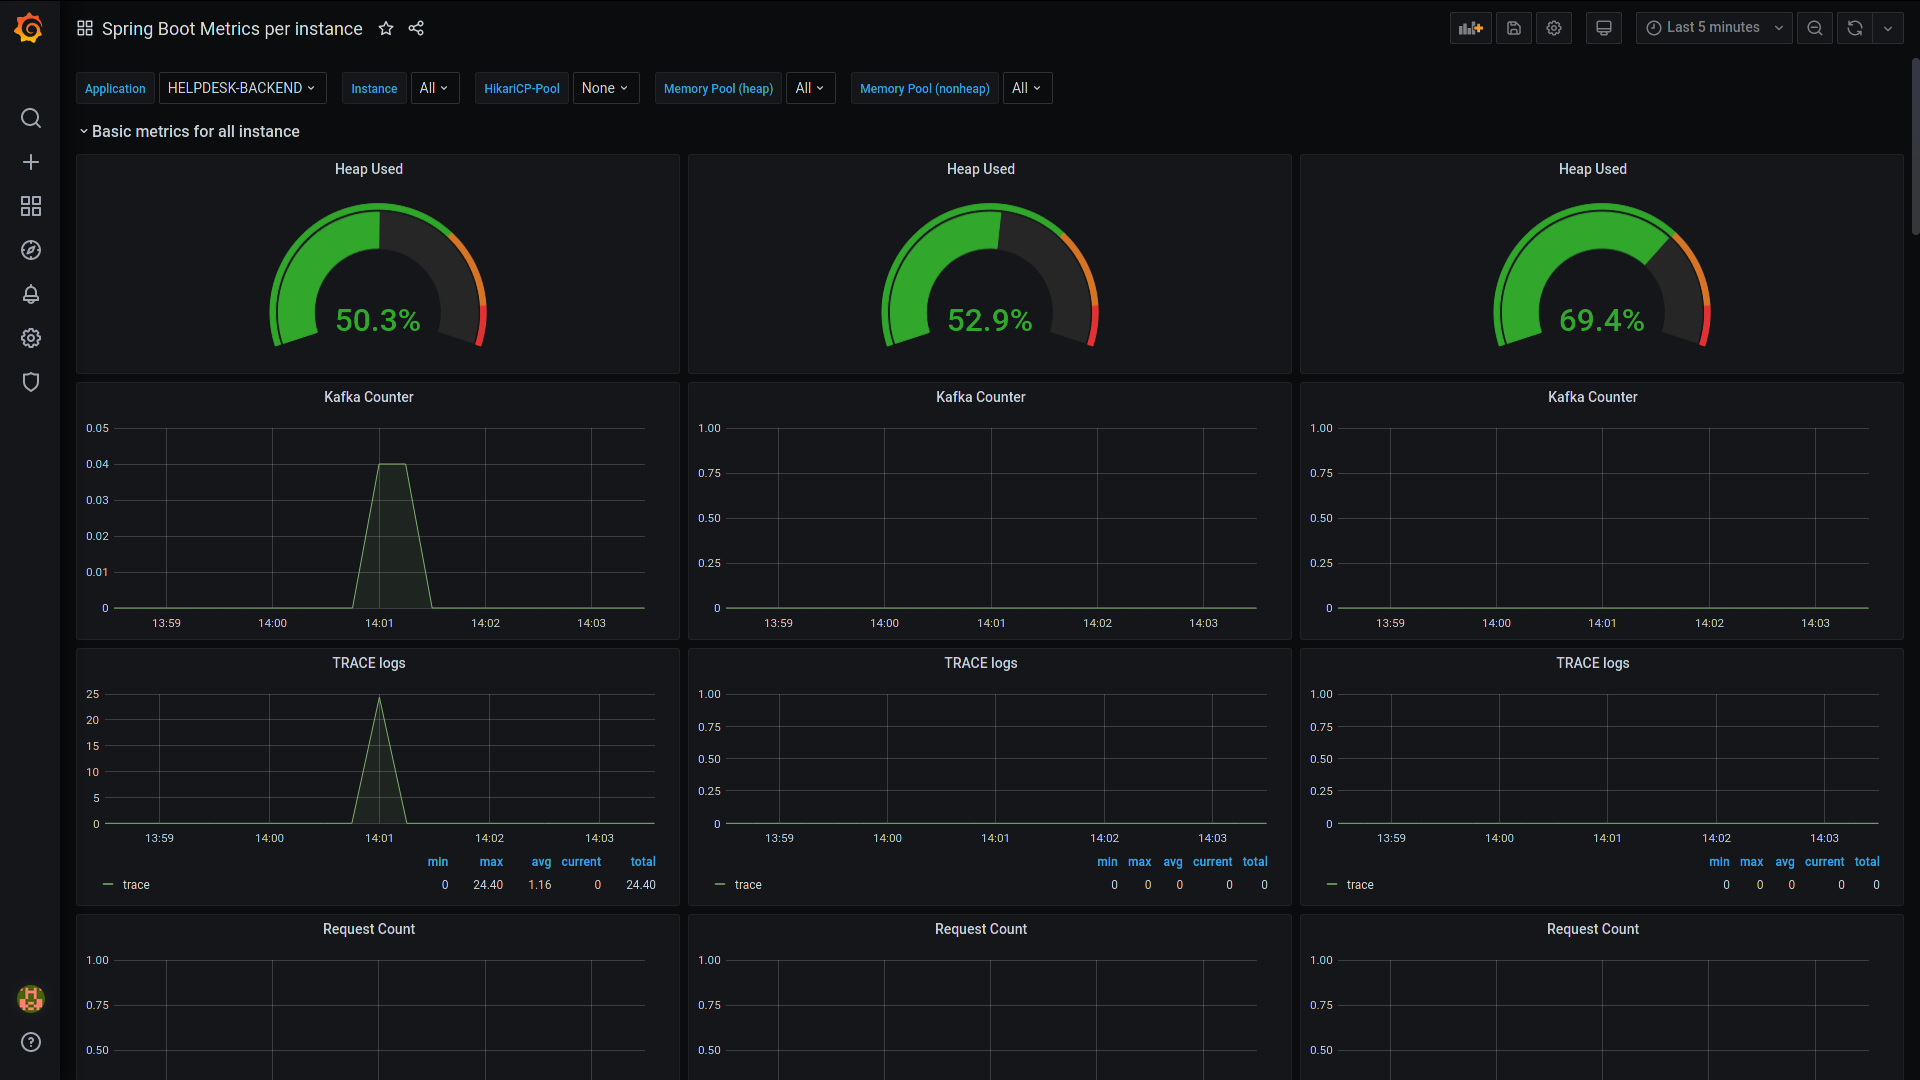
\includegraphics[width=.9\linewidth]{backend_receiving_email_from_kafka.png}  
		\caption{Az egyes instance kafka üzenet fogad}
		\label{fig:backend_receive_kafka}
	\end{subfigure}
	\begin{subfigure}{.49\textwidth}
		\centering
		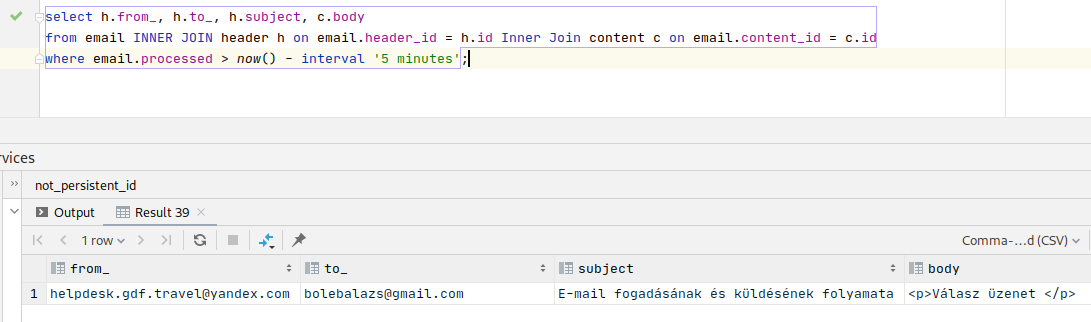
\includegraphics[width=.9\linewidth]{database_with_the_answer.png}  
		\caption{A válasz e-mail az adatbázisban}
		\label{fig:database_answer}
	\end{subfigure}

	\quad

\begin{subfigure}{.49\textwidth}
	\centering
	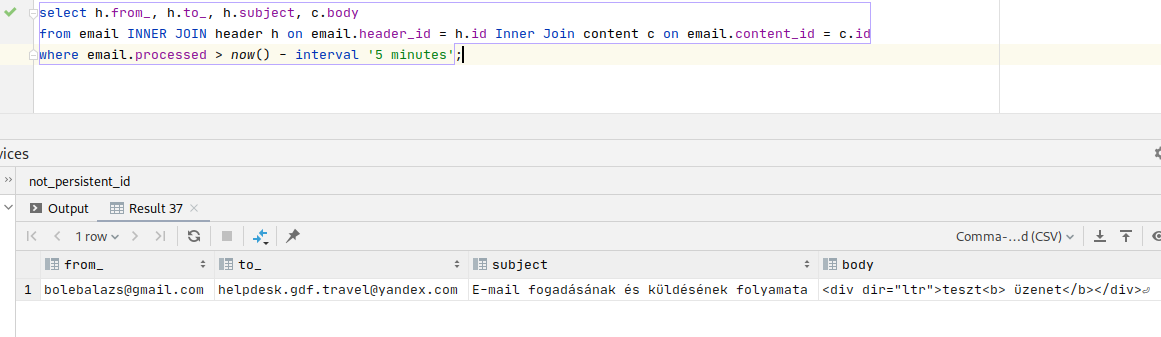
\includegraphics[width=.9\linewidth]{databse_incoming_email.png}  
	\caption{Az új e-mail az adatbázisban}
	\label{fig:datbase_received_email}
\end{subfigure}
\begin{subfigure}{.49\textwidth}
	\centering
	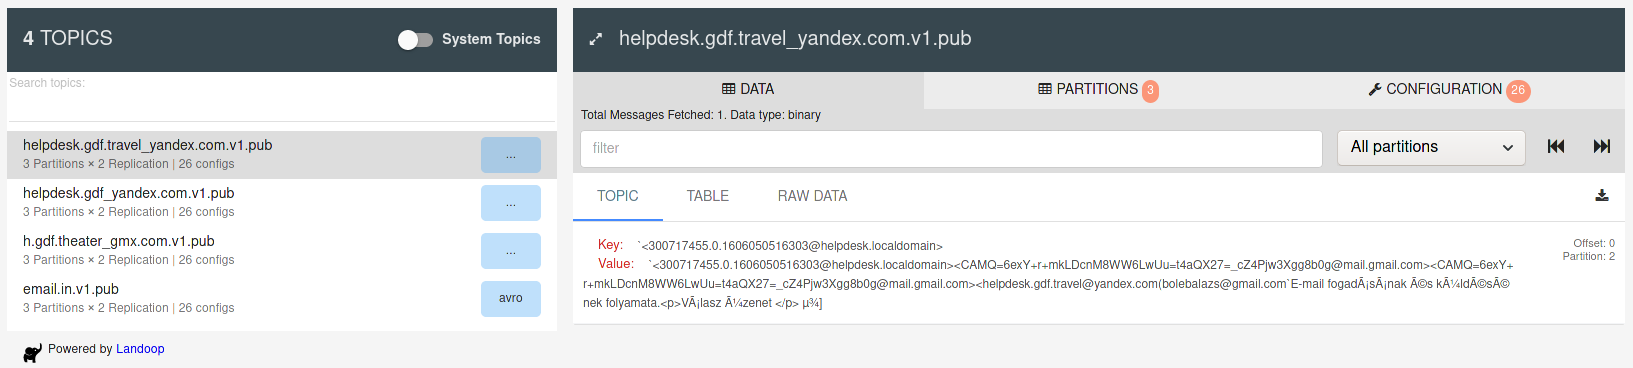
\includegraphics[width=.9\linewidth]{kafka_topic_with_the_sent_email.png}  
	\caption{A \textit{h.gdf.theater\textunderscore gmx.com.v1.pub} topic új üzenete}
	\label{fig:kafka_topic_send_email}
\end{subfigure}

	\quad

\begin{subfigure}{.45\textwidth}
	\centering
	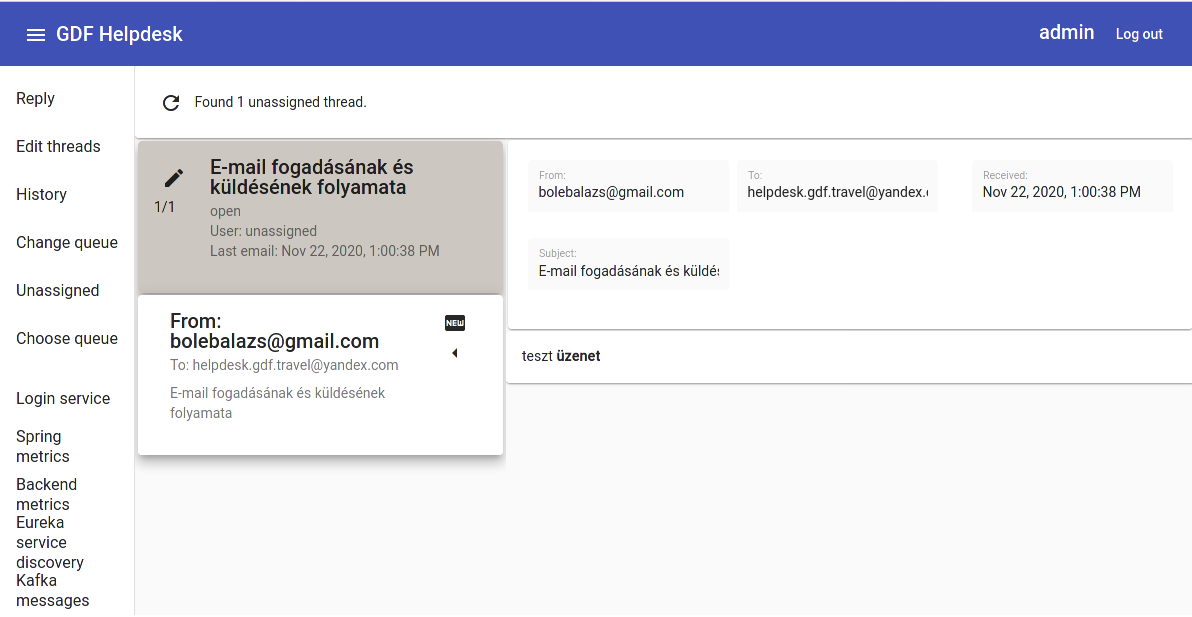
\includegraphics[width=.9\linewidth]{helpdesk_frontend_receive_incoming_email.png}  
	\caption{A felületen elérhető az új e-mail}
	\label{fig:frontend_read_email}
\end{subfigure}
\begin{subfigure}{.45\textwidth}
	\centering
	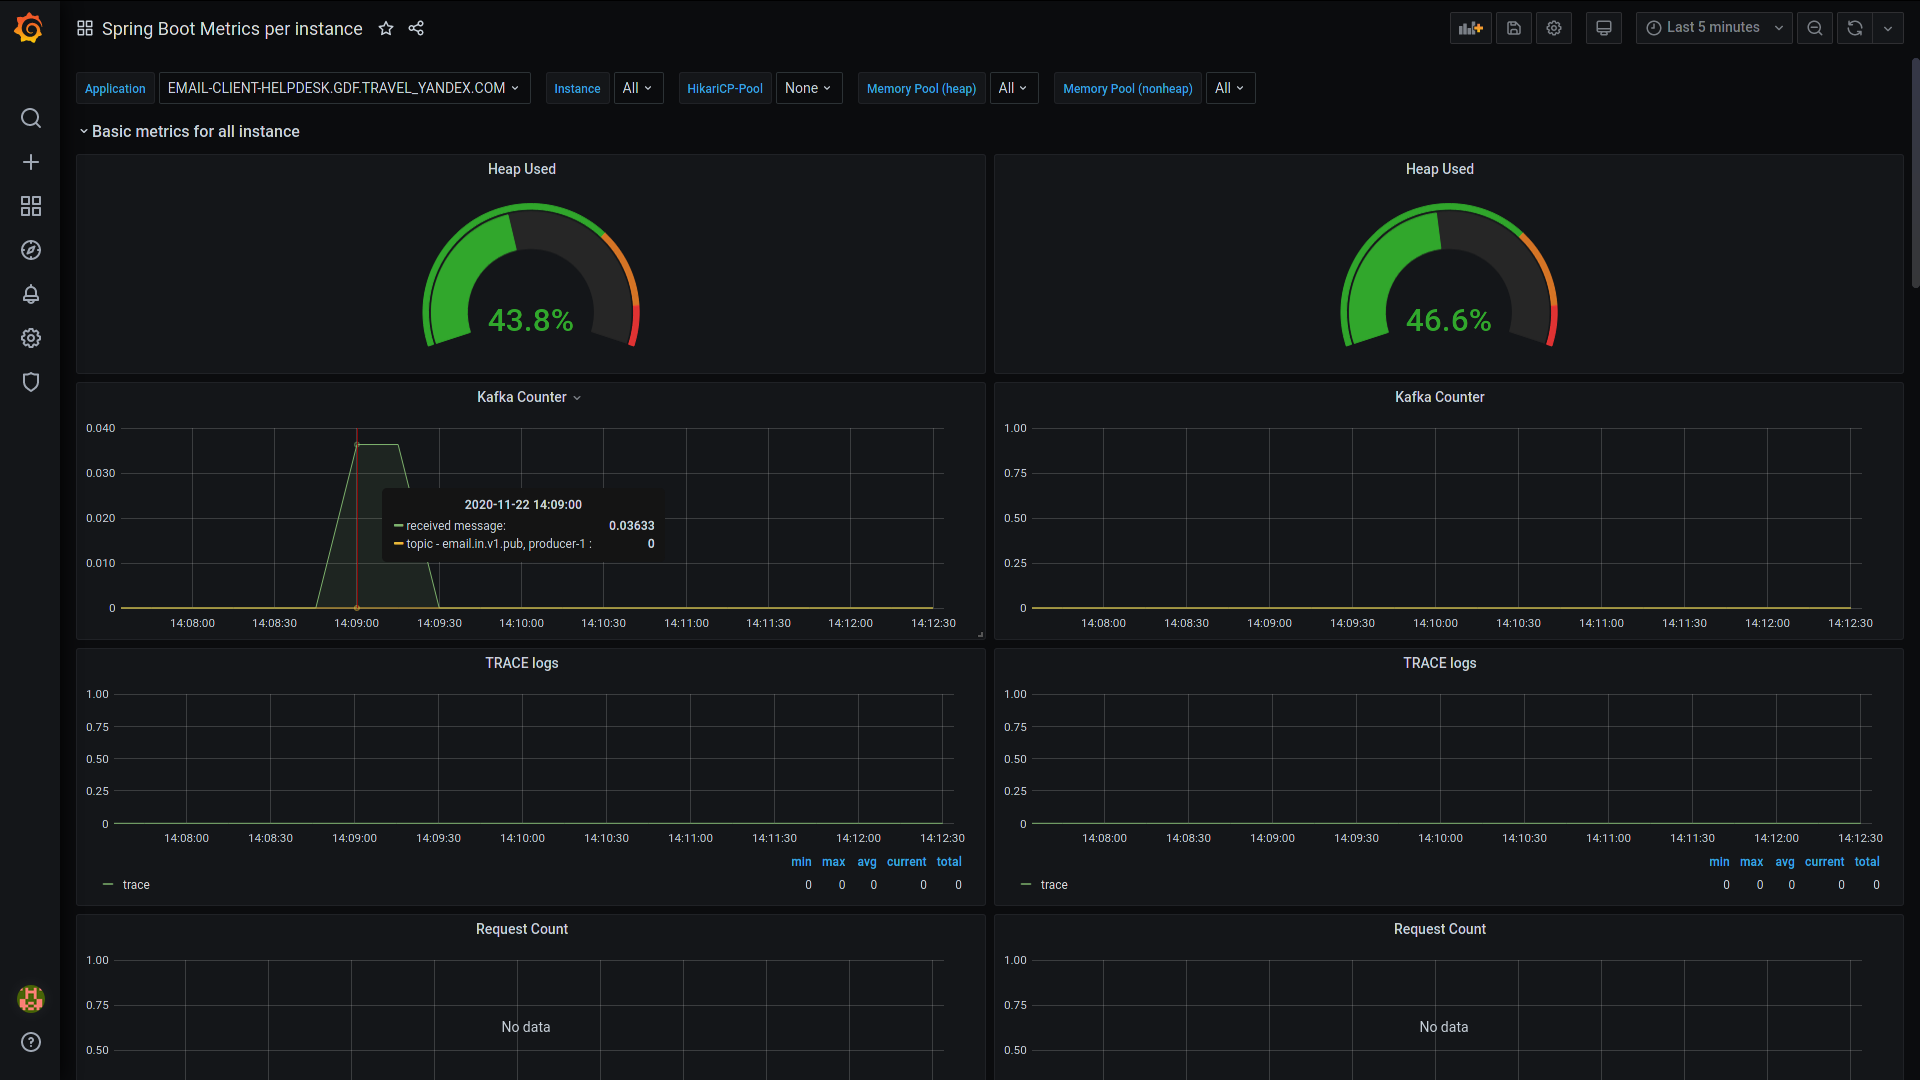
\includegraphics[width=.9\linewidth]{email_client_sending_email.png}  
	\caption{Az egyes instance kafka üzenet fogad}
	\label{fig:email_client_receives_kafka}
\end{subfigure}

	\caption[E-mail fogadásának és küldésének folyamata]{E-mail fogadásának és küldésének folyamata során követhető lépések}
	\label{fig:email_send_receive_visible}
\end{figure}



\section{Adatbázistáblák}
A helpdesk backend adatbázistábláit \aref{fig:extended_database_uml}. ábra tartalmazza.

\begin{figure}[hbt] 
	\centering
	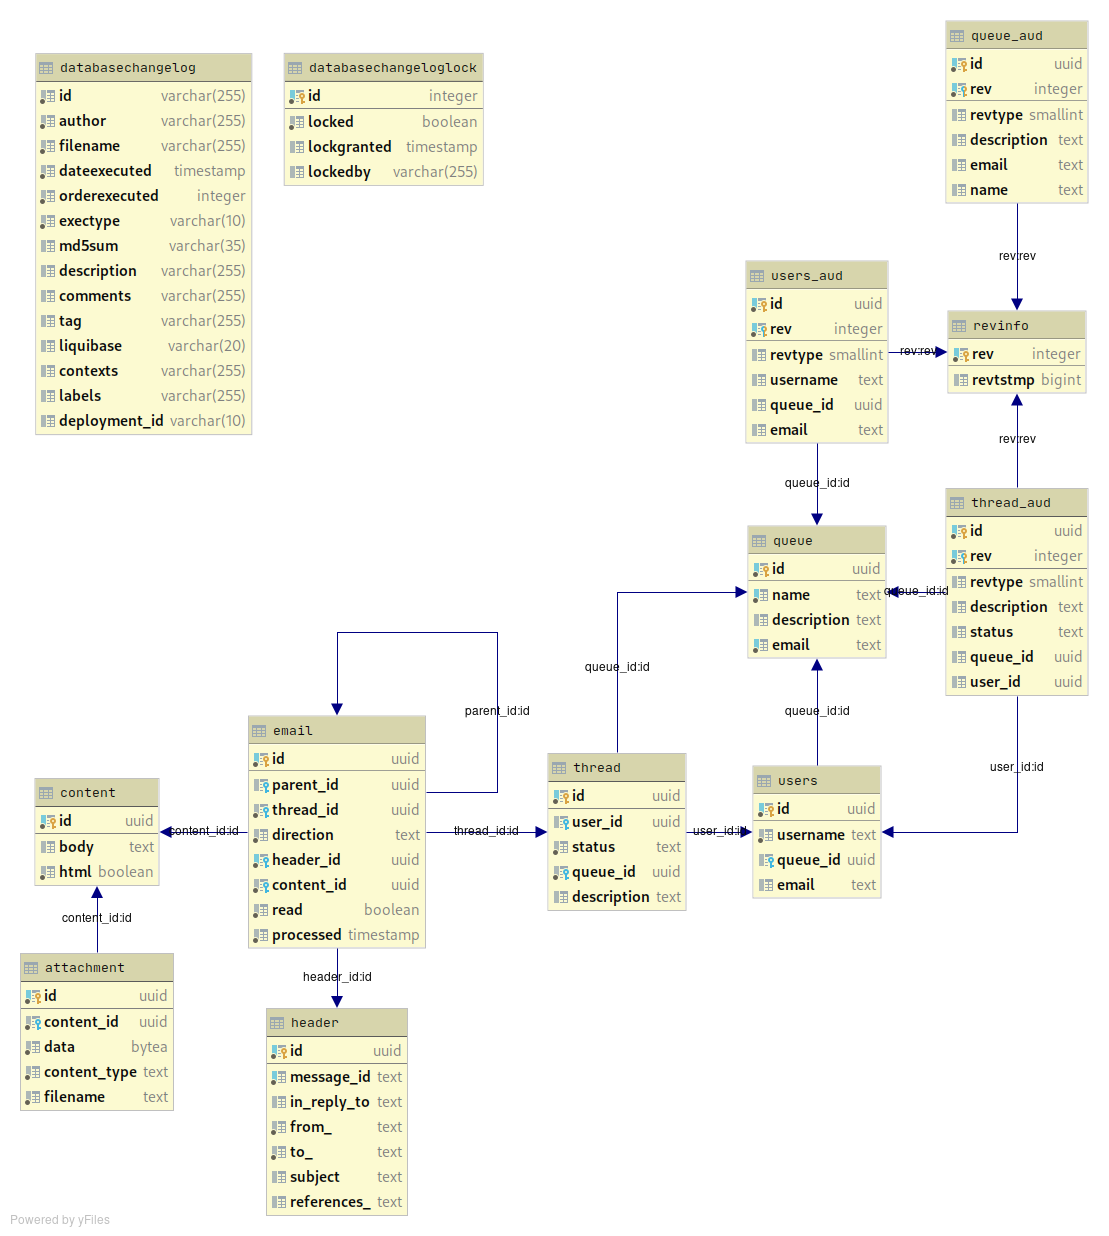
\includegraphics[width=0.85\textwidth]{extended_database_uml.png}
	\caption{A backend összes adatbázistáblája}
	\label{fig:extended_database_uml}
	\floatfoot{Forrás: saját ábra}
\end{figure}


\subsection{Liquibase}\label{sec:liquibase}
A \textit{databasechangelog} és \textit{databasechangeloglock} táblákat a Liquibase (\ref{sec:adatbazis}. pont) az adatbázis séma verziójának karbantartására használja:
\begin{description}
	\item[databasechangelog] tábla tartalmazza a \mbox{\textit{resources/db.changelog}} könyvtárban található,  \mbox{\textit{db.changelog-master.yaml}} állományban tárolt utasítások futási eredményeit.
	
	\item[databasechangeloglockot] minden végrehajtásnál a Liquibase példánya  zárolja, ezzel biztosítva hogy mindig maximum egy példány hajtson végre módosításokat az adatbázison (lásd \ref{sec:konkurencia_kezekese} pont, pesszimista konkurenciakezelési stratégia).
\end{description}

A helpdesk backend szerviz minden induláskor elindítja a Liquibase-t. A Liquibase csatlakozik az adatbázishoz a \textit{helpdesk} felhasználóval, és lefuttatja a \mbox{\textit{db.changelog-master.yaml}} állományban tárolt utasításokat.

A \mbox{\textit{db.changelog-master.yaml}} állományba fel van véve az összes olyan DDL-utasítás és más SQL-parancs, ami az adatbázis kezdő állapotának létrehozásához szükséges. Mivel a Liquibase ezeket a parancsokat a \textit{helpdesk} felhasználóval hajtja végre, a létrejött táblák is \textit{helpdesk} felhasználóhoz fognak tartozni. 

A helpdesk backend alkalmazás rendes működése során --  a Liquibase futása után --   a \textit{helpdesk\textunderscore app} felhasználón keresztül kapcsolódik az adatbázishoz, így csak a Liquibase utasításokban meghatározott táblákhoz fér hozzá, és csak olyan típusú --  CRUD --   utasítást tud végrehajtani, ami külön engedélyezve van neki.

Így biztosítható, hogy a helpdesk alkalmazás csak a feladatinak ellátásához szükséges szinten férjen hozzá az alkalmazáshoz, és hogy futása során ne módosíthassa a táblákat. 


\subsection{Hibernate Envers}\label{sec:hubernate_envers}
A \textit{revinfo} és az összes \textit{\textunderscore aud} végződésú táblát --  \textit{\mbox{users\textunderscore aud}, \mbox{queue\textunderscore aud} és \mbox{thread\textunderscore aud}} --   a Hibernate Envers használja az e-mail szál és a kapcsolódó entitások állapotának követésére.

\begin{description}
	\item[revinfo] tábla tartalmazza a módosítás időpontját és sorszámát.
	
	\item[\textunderscore aud] tábla tartalmazza a módosítás típusát, sorszámát és az entitás új értékeit.
\end{description}

Az Envers --  a \textit{Hibernate Event system}en keresztül --   figyeli, és feltartóztatja az e-mail szál állapotváltozásait. Hozzáadja a saját verziókövetéshez szükséges kódját, és csak akkor engedi sikeresen lezárni a tranzakciót, ha az \textunderscore aud tábla is sikeresen módosul.

Az Envers minden állapothoz eltárolja a módosítás típusát --  \textit{insert, update}, vagy \textit{delete} --   sorszámát és dátumát. Így mindig visszakereshető hogy melyik időpillanatban mi volt az entitás értéke.



\section{Apache Kafka}\label{sec:kafka_topics}
A kafka \textit{topic}ok és üzenetek elérhetőek és követhetőek a \textit{Kafka messages} menü pontja alatti Kafka Topics UI (\ref{fig:Kafka_Topics_UI}. ábra) eszközzel.

\begin{figure}[hbt] 
	\centering
	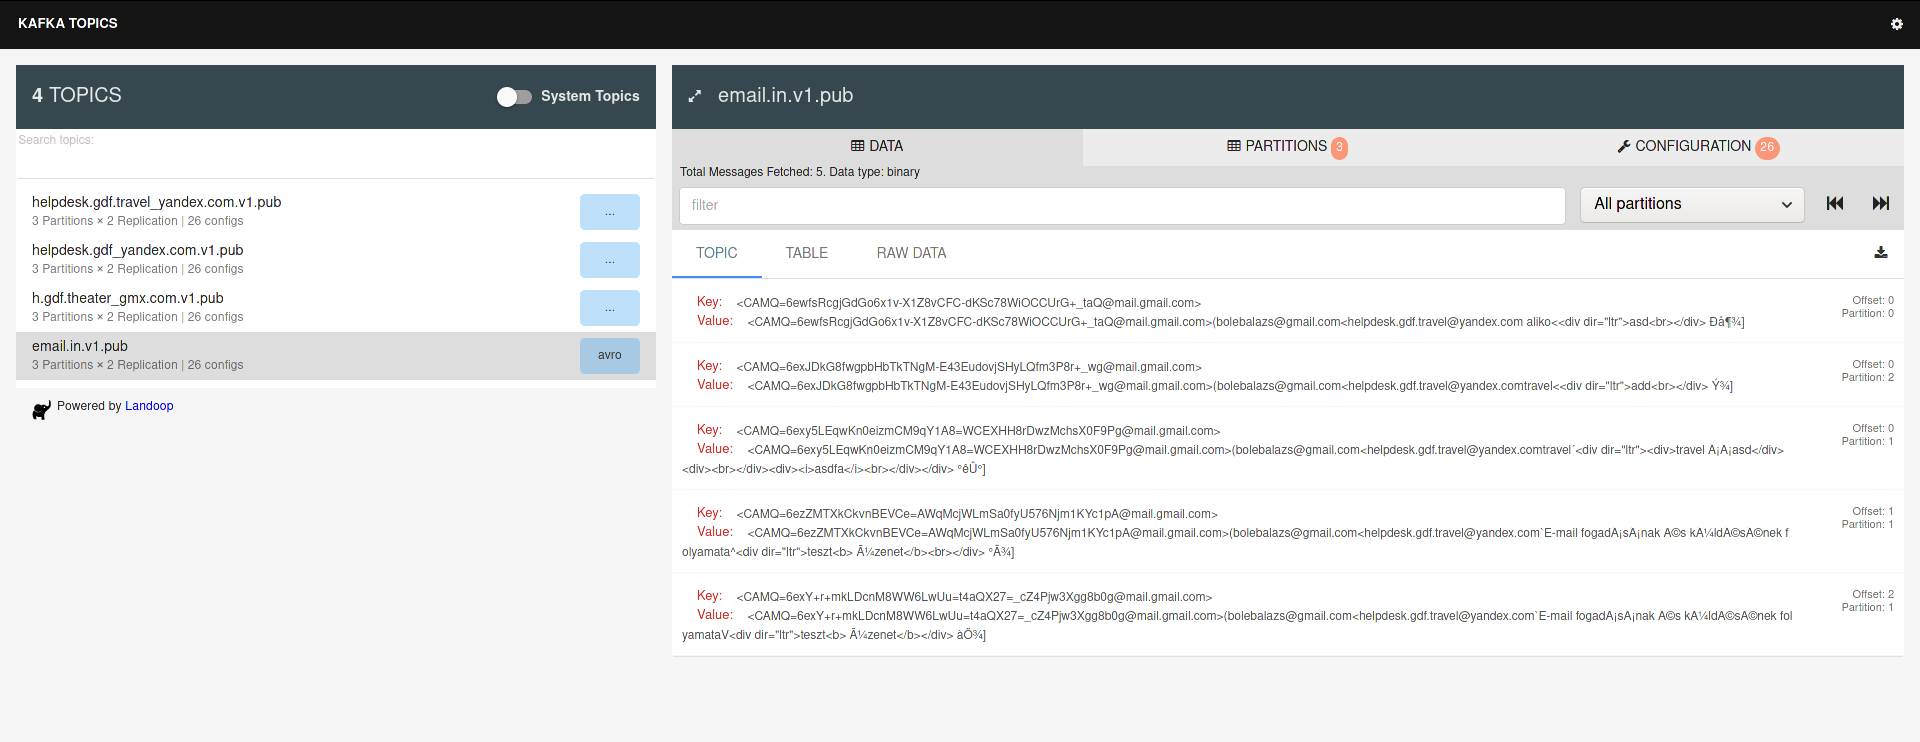
\includegraphics[width=0.9\textwidth]{Kafka_topic_ui.png}
	\caption[A Kafka Topics UI felülete]{A Kafka Topics UI eszközzel követhetőek a kafka \textit{topic}ok üzenetei, partíciói és beállításai}
	\label{fig:Kafka_Topics_UI}
	\floatfoot{Forrás: saját ábra}
\end{figure}


A helpdesk alakalmazás összesen hat \textit{topic}-ot használ:
\begin{description}
	\item[user.v1.pub] a Keycloak-ban regisztrált és karbantartott felhasználókat tartalmazza,
	
	\item[email.in.v1.pub] az összes beérkező  e-mailt tartalmazza,
	
	\item[helpdesk.gdf\textunderscore yandex.com.v1.pub] a  \href{mailto:helpdesk.gdf@yandex.com}{\nolinkurl{helpdesk.gdf@yandex.com}} címre küldött e-maileket tartalmazza,
	
	\item[helpdesk.gdf.travel\textunderscore yandex.com.v1.pub] a \href{mailto:helpdesk.gdf.travel@yandex.com}{\nolinkurl{helpdesk.gdf.travel@yandex.com}} címre küldött e-maileket tartalmazza,
	
	
	\item[h.gdf.theater\textunderscore gmx.com.v1.pub] a \href{mailto:h.gdf.theater@gmx.com}{\nolinkurl{h.gdf.theater@gmx.com}} címre küldött e-maileket tartalmazza,
	
	\item[\textunderscore schemas] a Schemaregistry ebben a \textit{topic}ban tárolja az alkalmazásban használt Avro schemákat.
\end{description}


Az alkalmazás három kafka brókert futtat egy clusterben. Továbbá minden üzleti funkcionalitást hordozó \textit{topic} --  a \textunderscore schemas-on kívül mindegyik --   három partícióval és kettes replikációs faktorral lett létrehozva.
Így a kafka cluster egy bróker kiesése, vagy egy partíció sérülése esetén is működőképes marad.


\section{Eureka}
\Aref{sec:metrikak}. pontban említett szerviz felderítésre az Eureka szervert használom. A helpdesk backend és az e-mail kliens az elindításuk után közvetlenül beregisztrálják magukat az Eureka szervizbe.

Az Eureka szerveren keresztül megtekinthető és más szervizek számára elérhető a példányok aktuális állapota és neve. Az oldal elérhető a \textit{Eureka service discovery} menüpont alatt~(\ref{fig:eureka}. ábra).


\begin{figure}[hbt] 
	\centering
	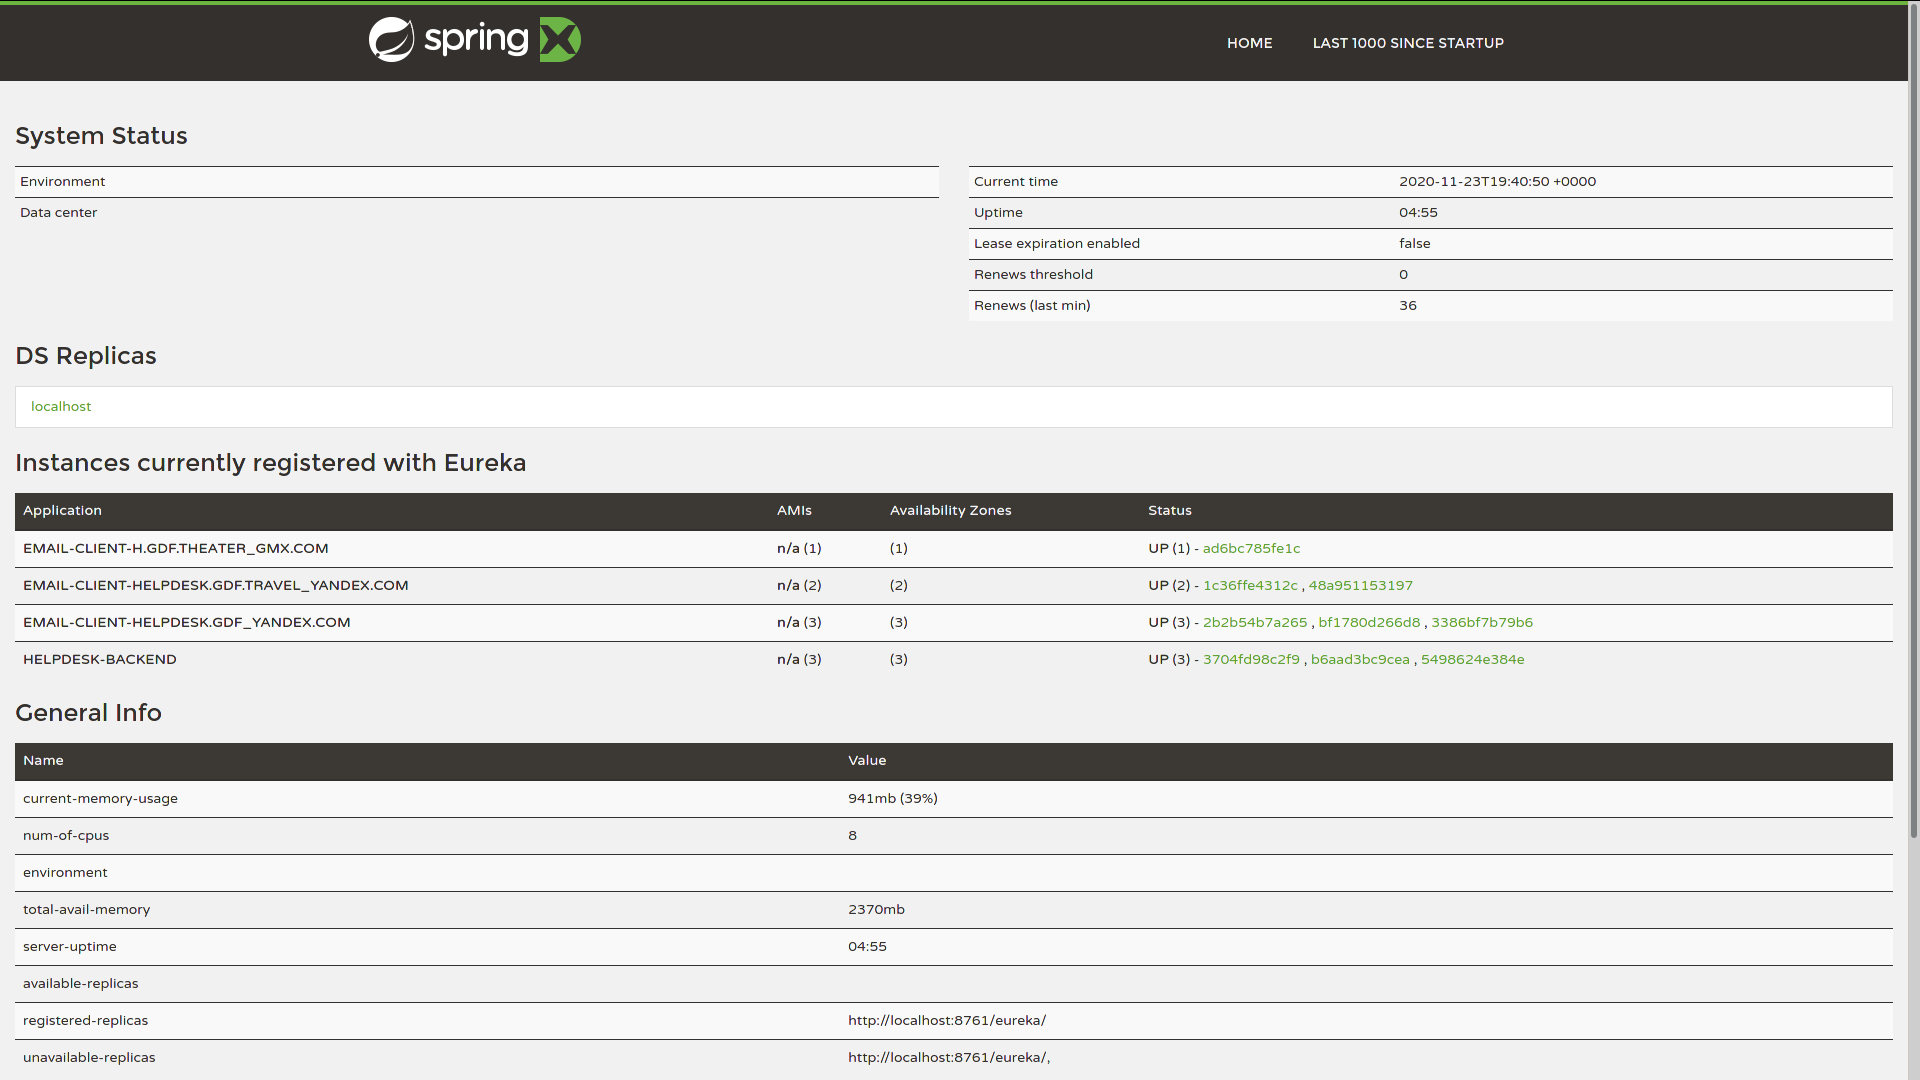
\includegraphics[width=0.85\textwidth]{eureka.png}
	\caption[Az Eureka service discovery felülete]{Az Eureka service discovery-n látható a mikroszerviz példányainak állapota és egyedi azonosítója}
	\label{fig:eureka}
	\floatfoot{Forrás: saját ábra}
\end{figure}




\chapter{Továbbfejlesztési lehetőségek}
\pagestyle{main}
\section{A deploymentről}

A helpdesk alkalmazás szervizei úgy lettek kialakítva, hogy képesek legyenek egymástól függetlenül, akár több példányban is működni. Ezáltal költséghatékonnyá téve a működést, leegyszerűsítve a hibatűrést, és lehetővé téve a változó terhelés miatti skálázhatóságot.

Azonban amíg a docker konténerek egy host gépen futnak és egy erőforráson osztoznak, soha nem lehet gazdaságosan megoldani a skálázást, és nem tud a rendszer felkészülni a számítógép kiesésére.

A következő logikus lépés tehát az alkalmazás \textit{cluster}re migrálása. A docker natívan támogatja a Microsoft Azure és az Amazon \cite{docker_website_deploy_ECS} szolgáltatókat. Így tehát a kód és a beállítások módosítása nélkül lehetséges az alkalmazás \textit{cluster}esítése docker swarmmal.

\bigskip
\section{A kódról}
A helpdesk alkalmazásba --  architektúrája miatt --   könnyű új funkciót fejleszteni. A most működő modulok mind lazán kapcsolódnak egymáshoz, így könnyű egy teljesen különböző, akár eltérő programnyelven íródott új funkció integrálása.

Mivel az összes technikai megkötés csupán a protokollok megvalósítása, nyugodtan lehet az új funkció tervezésénél a feladathoz választani a programnyelvet vagy a programozási módszertant is. 

Ha az új funkciónak szüksége lenne az alkalmazás más rendszeréhez tartozó adatára, akkor a kérdéses rendszer --  ahogy a Keycloak plugin példáján megmutattam --   ugyanúgy bővíthető, a komponensek közötti laza kapcsolat megőrizhető.

Hasonlóképpen, a laza kapcsolatok és jól definiált határok miatt, egyszerű egy-egy modult teljesen lecserélni, vagy más nyelven, más technológiával újraírni.

Mivel egy szerviz egy feladattal foglalkozik, ha például le	 kell cserélni a frontendet, akkor az új felhasználói felületen csak a megjelenítéssel kell foglalkozni, az üzleti funkciók megvalósítása a backend feladata, így azok továbbra is változatlanok maradnak.

Ugyanez nem csak a szervizek, hanem a kód szintjén is igaz. A hexagonális architektúra miatt, az adatbázis --  mint külső függőség --   könnyen cserélhető. 




\chapter{Tapasztalatok}
\pagestyle{main}
Szeretném összefoglalni a szakdolgozat készítése során nyert tapasztalataim.


nem funkcionális technológiák, mint git, latex

kutatómunka a tervezés hogy mwnnyi minden

a problémát analizálni és megfeelő megoldást keresni rá

a végé pedig hogy ez mennyire csodás érzés hogy minden úgy működik ahogy kitaláltam.


meg miket tanultam:
normalizálás adatbázis
spring  angular
dependency injection



\chapter*{Összefoglalás}\label{ch:osszefoglalas}
\pagestyle{plain}
összefoglalás a végén

meg miket tanultam:
normalizálás adatbázis
spring  angular
dependency injection

\newpage


% References
\bibliographystyle{unsrturl}
\bibliography{references.bib}



\end{document}
